% !TeX document-id = {af928648-7a45-486b-aa45-9066bfc9e040}
% !TeX spellcheck = en-US
% !TeX encoding = utf8
% !TeX program = pdflatex
% !BIB program = biber

\let\ifdeutsch\iffalse
\let\ifenglisch\iftrue
% EN: This file is loaded before the \documentclass command in the main document

% EN: The following package allows \\ at the title page
%     For more information see https://github.com/latextemplates/scientific-thesis-cover/issues/4
\RequirePackage{kvoptions-patch}

\ifenglisch
  \PassOptionsToClass{numbers=noenddot}{scrbook}
\else
  %()Aus scrguide.pdf - der Dokumentation von KOMA-Script)
  %Nach DUDEN steht in Gliederungen, in denen ausschließlich arabische Ziffern für die Nummerierung
  %verwendet werden, am Ende der Gliederungsnummern kein abschließender Punkt
  %(siehe [DUD96, R3]). Wird hingegen innerhalb der Gliederung auch mit römischen Zahlen
  %oder Groß- oder Kleinbuchstaben gearbeitet, so steht am Ende aller Gliederungsnummern ein
  %abschließender Punkt (siehe [DUD96, R4])
  \PassOptionsToClass{numbers=autoendperiod}{scrbook}
\fi

% Warns about outdated packages and missing caption declarations
% See https://www.ctan.org/pkg/nag
\RequirePackage[l2tabu, orthodox]{nag}

%DE: Neue deutsche Trennmuster
%    Siehe http://www.ctan.org/pkg/dehyph-exptl und http://projekte.dante.de/Trennmuster/WebHome
%    Nur für pdflatex, nicht für lualatex
\RequirePackage{ifluatex}
\ifluatex
  % do not load anything
\else
  \ifdeutsch
    \RequirePackage[ngerman=ngerman-x-latest]{hyphsubst}
  \fi
\fi

\documentclass[
a4paper,
twoside,
% bibliography=totoc,
% dxtotoc,   %Index ins Inhaltsverzeichnis
% liststotoc, %List of X ins Inhaltsverzeichnis, mit liststotocnumbered werden die Abbildungsverzeichnisse nummeriert
headsepline,
cleardoublepage=empty,
parskip=half,
% draft um zu sehen, wo noch nachgebessert werden muss - wichtig, da Bindungskorrektur mit drin
draft=false
]{scrbook}
% !TeX encoding = utf8

% EN: This file includes basic packages and sets options. The order of package
%     loading is important
% DE: In dieser Datei werden zuerst die benoetigten Pakete eingebunden und
%     danach diverse Optionen gesetzt. Achtung Reihenfolge ist entscheidend!


%%%
% EN: Styleguide:
% - English comments are prefixed with "EN", German comments are prefixed with "DE"
% - Prefixed headings define the language for the subsequent paragraphs
% - It is tried to organize packages in blocks. One block starts with %%%, then
%   % <heading>, then the options and more text. % followed by %%% end a block.
%
% DE: Styleguide:
%
% Ein sehr kleiner Styleguide. Packages werden in Blöcken organisiert.
% Ein Block beginnt mit drei % in einer Zeile, dann % <Blocküberschrift>, dann
% eine Liste der möglichen Optionen und deren Einstellungen, Gründe und Kommentare
% eine % Zeile in der sonst nichts steht und dann wieder %%% in einer Zeile.
%
% Zwischen zwei Blöcken sind 2 Leerzeilen!
% Zu jedem Paket werden soviele Optionen wie möglich/nötig angegeben
%
%%%

%%%
% EN: File encoding
% DE: Codierung
%     Wir sind im 21 Jahrhundert, utf-8 löst so viele Probleme.
%
% Mit UTF-8 funktionieren folgende Pakete nicht mehr. Bitte beachten!
%   * fancyvrb mit §
%   * easylist -> http://www.ctan.org/tex-archive/macros/latex/contrib/easylist/
\ifluatex
  %no package loading required
\else
  \usepackage[utf8]{inputenc}
\fi
%
%%%

%%%
% DE: Parallelbetrieb tex4ht und pdflatex
\makeatletter
\@ifpackageloaded{tex4ht}{
  \def\iftex4ht{\iftrue}
}{
  \def\iftex4ht{\iffalse}
}
\makeatother
%%%


%%%
% EN: Defintion of colors
% DE: Farbdefinitionen
\usepackage[hyperref,dvipsnames]{xcolor}
%

%%%
% EN: Required for custom acronyms/glossaries style.
%     Left aligned Columns in tables with fixed width.
%     See http://tex.stackexchange.com/questions/91566/syntax-similar-to-centering-for-right-and-left
\usepackage{ragged2e}
%%%

%%%
% Abkürzungsverzeichnis
\usepackage{scrwfile} % Wichtig, ansonsten erscheint "No room for a new \write"
% siehe http://www.dickimaw-books.com/cgi-bin/faq.cgi?action=view&categorylabel=glossaries#glsnewwriteexceeded
\usepackage[acronym,indexonlyfirst,nomain]{glossaries}
\ifdeutsch
  \renewcommand*{\acronymname}{Abkürzungsverzeichnis}
\else
  \renewcommand*{\acronymname}{List of Abbreviations}
\fi
\renewcommand*{\glsgroupskip}{}
%
% Removed Glossarie as a table as a quick fix to get the template working again
% see http://tex.stackexchange.com/questions/145579/how-to-print-acronyms-of-glossaries-into-a-table
%
\makenoidxglossaries
%%%


%%%
% EN: Support for language-specific hyphenation
% DE: Neue deutsche Rechtschreibung und Literatur statt "Literature"
%     Die folgende Einstellung ist der Nachfolger von ngerman.sty
\ifdeutsch
  % DE: letzte Sprache ist default, Einbindung von "american" ermöglicht \begin{otherlanguage}{amercian}...\end{otherlanguage} oder \foreignlanguage{american}{Text in American}
  %     Siehe auch http://tex.stackexchange.com/a/50638/9075
  \usepackage[american,ngerman]{babel}
  % Ein "abstract" ist eine "Kurzfassung", keine "Zusammenfassung"
  \addto\captionsngerman{%
    \renewcommand\abstractname{Kurzfassung}%
  }
\else
  %
  %
  % EN: if you are writing in English
  %     last language is the default language
  \usepackage[ngerman,american]{babel}
\fi
%
%%%

%%%
% Anführungszeichen
% Zitate in \enquote{...} setzen, dann werden automatisch die richtigen Anführungszeichen verwendet.
\usepackage{csquotes}
%%%


%%%
% EN: extended enumarations
% DE: erweitertes Enumerate
\usepackage{paralist}
%
%%%


%%%
% fancyheadings (nicht nur) fuer koma
\usepackage[automark]{scrlayer-scrpage}
%
%%%


%%%
% EN: Mathematics
% DE: Mathematik
%
\usepackage[]{amsmath} % Viele Mathematik-Sachen: Doku: /usr/share/doc/texmf/latex/amsmath/amsldoc.dvi.gz
\PassOptionsToPackage{fleqn,leqno}{amsmath} % options must be passed this way, otherwise it does not work with glossaries
%fleqn (=Gleichungen linksbündig platzieren) funktioniert nicht direkt. Es muss noch ein Patch gemacht werden:
%\addtolength\mathindent{1em}%work-around ams-math problem with align and 9 -> 10. Does not work with glossaries, No visual changes.
\usepackage{mathtools} %fixes bugs in AMS math
%
%for theorems, replacement for amsthm
\usepackage[amsmath,hyperref]{ntheorem}
\theorempreskipamount 2ex plus1ex minus0.5ex
\theorempostskipamount 2ex plus1ex minus0.5ex
\theoremstyle{break}
\newtheorem{definition}{Definition}[section]
%
%%%


%%%
% Intelligentes Leerzeichen um hinter Abkürzungen die richtigen Abstände zu erhalten, auch leere.
% siehe commands.tex \gq{}
\usepackage{xspace}
%Macht \xspace und \enquote kompatibel
\makeatletter
\xspaceaddexceptions{\grqq \grq \csq@qclose@i \} }
\makeatother
%
%%%


%%%
% EN: Package for the appendix
% DE: Anhang
\usepackage{appendix}
%[toc,page,title,header]
%
%%%

%%%
% EN: Graphics
% DE: Grafikeinbindungen
%
% EN: The parameter "pdftex" is not required
\usepackage{graphicx}
\graphicspath{{\getgraphicspath}}
\newcommand{\getgraphicspath}{graphics/}
%
%%%


%%%
% Enables inclusion of SVG graphics - 1:1 approach
% This is NOT the approach of http://www.ctan.org/tex-archive/info/svg-inkscape,
% which allows text in SVG to be typeset using LaTeX
% We just include the SVG as is
\usepackage{epstopdf}
\epstopdfDeclareGraphicsRule{.svg}{pdf}{.pdf}{%
  inkscape -z -D --file=#1 --export-pdf=\OutputFile
}
%
%%%


%%%
% Enables inclusion of SVG graphics - text-rendered-with-LaTeX-approach
% This is the approach of http://www.ctan.org/tex-archive/info/svg-inkscape,
\newcommand{\executeiffilenewer}[3]{%
  \IfFileExists{#2}
  {
    %\message{file #2 exists}
    \ifnum\pdfstrcmp{\pdffilemoddate{#1}}%
      {\pdffilemoddate{#2}}>0%
      {\immediate\write18{#3}}
    \else
      {%\message{file up to date #2}
      }
    \fi%
  }{
    %\message{file #2 doesn't exist}
    %\message{argument: #3}
    %\immediate\write18{echo "test" > xoutput.txt}
    \immediate\write18{#3}
  }
}
\newcommand{\includesvg}[1]{%
  \executeiffilenewer{#1.svg}{#1.pdf}%
  {
    inkscape -z -D --file=\getgraphicspath#1.svg %
    --export-pdf=\getgraphicspath#1.pdf --export-latex}%
  \input{\getgraphicspath#1.pdf_tex}%
}


%%%
% EN: Enable typesetting values with SI units.
\usepackage{siunitx}
%%%

%%%
% EN: Extensions for tables
% DE: Tabellenerweiterungen
\usepackage{array} %increases tex's buffer size and enables ``>'' in tablespecs
\usepackage{longtable}
\usepackage{dcolumn} %Aligning numbers by decimal points in table columns
\ifdeutsch
  \newcolumntype{d}[1]{D{.}{,}{#1}}
\else
  \newcolumntype{d}[1]{D{.}{.}{#1}}
\fi
\setlength{\extrarowheight}{1pt}
%%%

%%%
% Eine Zelle, die sich über mehrere Zeilen erstreckt.
% Siehe Beispieltabelle in Kapitel 2
\usepackage{multirow}
%
%%%

%%%
%Fuer Tabellen mit Variablen Spaltenbreiten
%\usepackage{tabularx}
%\usepackage{tabulary}
%
%%%


%%%
% EN: Links behave as they should. Enables "\url{...}" for URL typesettings.
%     Allow URL breaks also at a hyphen, even though it might be confusing: Is the "-" part of the address or just a hyphen?
%     See https://tex.stackexchange.com/a/3034/9075.
% DE: Links verhalten sich so, wie sie sollen
%     Zeilenumbrüche bei URLs auch bei Bindestrichen erlauben, auch wenn es verwirrend sein könnte: Gehört der Bindestrich zur URL oder ist es ein Trennstrich?
%     Siehe https://tex.stackexchange.com/a/3034/9075.
\usepackage[hyphens]{url}
%
%  EN: When activated, use text font as url font, not the monospaced one.
%      For all options see https://tex.stackexchange.com/a/261435/9075.
% \urlstyle{same}
%
% EN: Hint by http://tex.stackexchange.com/a/10419/9075.
\makeatletter
\g@addto@macro{\UrlBreaks}{\UrlOrds}
\makeatother
%
%%%


%%%
% Index über Begriffe, Abkürzungen
%\usepackage{makeidx} makeidx ist out -> http://xindy.sf.net verwenden
%
%%%

%%%
%lustiger Hack fuer das Abkuerzungsverzeichnis
%nach latex durchlauf folgendes ausfuehren
%makeindex ausarbeitung.nlo -s nomencl.ist -o ausarbeitung.nls
%danach nochmal latex
%\usepackage{nomencl}
%    \let\abk\nomenclature %Deutsche Ueberschrift setzen
%          \renewcommand{\nomname}{List of Abbreviations}
%        %Punkte zw. Abkuerzung und Erklaerung
%          \setlength{\nomlabelwidth}{.2\hsize}
%          \renewcommand{\nomlabel}[1]{#1 \dotfill}
%        %Zeilenabstaende verkleinern
%          \setlength{\nomitemsep}{-\parsep}
%    \makenomenclature
%
%%%

%%%
% EN: Logic for TeX - enables if-then-else in commands
% DE: Logik für TeX
%     FÜr if-then-else @ commands.tex
\usepackage{ifthen}
%
%%%


%%%
% EN: Code Listings
% DE: Listings
\usepackage{listings}
\lstset{language=XML,
  showstringspaces=false,
  extendedchars=true,
  basicstyle=\footnotesize\ttfamily,
  commentstyle=\slshape,
  % DE: Original: \rmfamily, damit werden die Strings im Quellcode hervorgehoben. Zusaetzlich evtl.: \scshape oder \rmfamily durch \ttfamily ersetzen. Dann sieht's aus, wie bei fancyvrb
  stringstyle=\ttfamily, 
  breaklines=true,
  breakatwhitespace=true,
  % EN: alternative: fixed
  columns=flexible,
  numbers=left,
  numberstyle=\tiny,
  basewidth=.5em,
  xleftmargin=.5cm,
  % aboveskip=0mm, %DE: deaktivieren, falls man lstlistings direkt als floating object benutzt (\begin{lstlisting}[float,...])
  % belowskip=0mm, %DE: deaktivieren, falls man lstlistings direkt als floating object benutzt (\begin{lstlisting}[float,...])
  captionpos=b
}

\ifdeutsch
  \renewcommand{\lstlistlistingname}{Verzeichnis der Listings}
\fi
%
%%%


%%%
% EN: Alternative to listings could be fancyvrb. Can be used together.
% DE: Alternative zu Listings ist fancyvrb. Kann auch beides gleichzeitig benutzt werden.
\usepackage{fancyvrb}
%
%EN: Font size for the normal text
%DE: Groesse fuer den Fliesstext. Falls deaktiviert: \normalsize
%\fvset{fontsize=\small}
%
%DE: Somit kann im Text ganz einfach §verbatim§ text gesetzt werden.
%    Disabled, because UTF-8 does not work any more and lualatex causes issues
%\DefineShortVerb{\§}
%
%EN: Shrink font size of listings
\RecustomVerbatimEnvironment{Verbatim}{Verbatim}{fontsize=\footnotesize}
\RecustomVerbatimCommand{\VerbatimInput}{VerbatimInput}{fontsize=\footnotesize}
%
%EN: Hack for fancyvrb based on http://newsgroups.derkeiler.com/Archive/Comp/comp.text.tex/2008-12/msg00075.html
%EN: Change of the solution: \Vref somehow collidated with cleveref/varioref as the output of \Vref{} was "Abschnitt 4.3 auf Seite 85"; therefore changed to \myVref -- so completely removed
\newcommand{\Vlabel}[1]{\label[line]{#1}\hypertarget{#1}{}}
\newcommand{\lref}[1]{\hyperlink{#1}{\FancyVerbLineautorefname~\ref*{#1}}}
%
%%%


%%%
% EN: Tunings of captions for floats, listings, ...
% DE: Bildunterschriften bei floats genauso formatieren wie bei Listings
%     Anpassung wird unten bei den newfloat-Deklarationen vorgenommen
%     https://www.ctan.org/pkg/caption2 is superseeded by this package.
\usepackage{caption}
%
%%%


%%%
% EN: Provides rotating figures, where the PDF page is also turned
% DE: Ermoeglicht es, Abbildungen um 90 Grad zu drehen
%     Alternatives Paket: rotating Allerdings wird hier nur das Bild gedreht, während bei lscape auch die PDF-Seite gedreht wird.
%     Das Paket lscape dreht die Seite auch nicht
\usepackage{pdflscape}
%
%%%


%%%
%EN: Required for proper environments of fancyvrb and lstlistings
%    There is also the newfloat pacakge (recommended by minted), but we currently have no expericene with that
%DE: Wird für fancyvrb und für lstlistings verwendet
\usepackage{float}
%
% EN: Alternative to float package
%\usepackage{floatrow}
%DE: zustäzlich für den Paramter [H] = Floats WIRKLICH da wo sie deklariert wurden paltzieren - ganz ohne Kompromisse
%    floatrow ist der Nachfolger von float
%    Allerdings macht floatrow in manchen Konstellationen Probleme. Deshalb ist das Paket deaktiviert.
%
% EN: See http://www.tex.ac.uk/cgi-bin/texfaq2html?label=floats
% DE: floats IMMER nach einer Referenzierung platzieren
%\usepackage{flafter}
%%%


%%%
% EN: For nested figures
% DE: Fuer Abbildungen innerhalb von Abbildungen
%     Ersetzt die Pakete subfigure und subfig - siehe https://tex.stackexchange.com/a/13778/9075
\usepackage[hypcap=true]{subcaption}
%
%%%


%%%
% EN: Extended support for footnotes
% DE: Fußnoten
%
%\usepackage{dblfnote}  %Zweispaltige Fußnoten
%
% Keine hochgestellten Ziffern in der Fußnote (KOMA-Script-spezifisch):
%\deffootnote[1.5em]{0pt}{1em}{\makebox[1.5em][l]{\bfseries\thefootnotemark}}
%
% Abstand zwischen Fußnoten vergrößern:
%\setlength{\footnotesep}{.85\baselineskip}
%
% EN: Following command disables the separting line of the footnote
% DE: Folgendes Kommando deaktiviert die Trennlinie zur Fußnote
%\renewcommand{\footnoterule}{}
%
\addtolength{\skip\footins}{\baselineskip} % Abstand Text <-> Fußnote
%
% Fußnoten immer ganz unten auf einer \raggedbottom-Seite
% fnpos kommt aus dem yafoot package
\usepackage{fnpos}
\makeFNbelow
\makeFNbottom
%
%%%


%%%
% EN: Variable page heights
% DE: Variable Seitenhöhen zulassen
\raggedbottom
%
%%%


%%%
% Falls die Seitenzahl bei einer Referenz auf eine Abbildung nur dann angegeben werden soll,
% falls sich die Abbildung nicht auf der selben Seite befindet...
\iftex4ht
  %tex4ht does not work well with vref, therefore we emulate vref behavior
  \newcommand{\vref}[1]{\ref{#1}}
\else
  \ifdeutsch
    \usepackage[ngerman]{varioref}
  \else
    \usepackage{varioref}
  \fi
\fi
%%%

%%%
% EN: More beautiful tables if one uses \toprule, \midrule, \bottomrule
% DE: Noch schoenere Tabellen als mit booktabs mit http://www.zvisionwelt.de/downloads.html
\usepackage{booktabs}
%
%\usepackage[section]{placeins}
%
%%%


%%%
% EN: Graphs and Automata
%
% TODO: Since version 3.0 (2013-10-01), it supports pdflatex via the auto-pst-pdf package
%       Requires -shell-escape
%\usepackage{gastex}
%%%


%%%
%
%\usepackage{multicol}
%\usepackage{setspace} % kollidiert mit diplomarbeit.sty
%%%


%%%
%biblatex statt bibtex
\usepackage[
  backend       = biber, %biber does not work with 64x versions alternative: bibtex8
  %minalphanames only works with biber backend
  sortcites     = true,
  bibstyle      = alphabetic,
  citestyle     = alphabetic,
  firstinits    = true,
  useprefix     = false, %"von, van, etc." will be printed, too. See below.
  minnames      = 1,
  minalphanames = 3,
  maxalphanames = 4,
  maxbibnames   = 99,
  maxcitenames  = 3,
  natbib        = true,
  eprint        = true,
  url           = true,
  doi           = true,
  isbn          = true,
  backref       = true]{biblatex}

% enable more breaks at URLs. See https://tex.stackexchange.com/a/134281.
\setcounter{biburllcpenalty}{7000}
\setcounter{biburlucpenalty}{8000}

\bibliography{bibliography}
%\addbibresource[datatype=bibtex]{bibliography.bib}

%Do not put "vd" in the label, but put it at "\citeauthor"
%Source: http://tex.stackexchange.com/a/30277/9075
\makeatletter
\AtBeginDocument{\toggletrue{blx@useprefix}}
\AtBeginBibliography{\togglefalse{blx@useprefix}}
\makeatother

%Thin spaces between initials
%http://tex.stackexchange.com/a/11083/9075
\renewrobustcmd*{\bibinitdelim}{\,}

%Keep first and last name together in the bibliography
%http://tex.stackexchange.com/a/196192/9075
\renewcommand*\bibnamedelimc{\addnbspace}
\renewcommand*\bibnamedelimd{\addnbspace}

%Replace last "and" by comma in bibliography
%See http://tex.stackexchange.com/a/41532/9075
\AtBeginBibliography{%
  \renewcommand*{\finalnamedelim}{\addcomma\space}%
}

\DefineBibliographyStrings{ngerman}{
  backrefpage  = {zitiert auf S\adddot},
  backrefpages = {zitiert auf S\adddot},
  andothers    = {et\ \addabbrvspace al\adddot},
  %Tipp von http://www.mrunix.de/forums/showthread.php?64665-biblatex-Kann-%DCberschrift-vom-Inhaltsverzeichnis-nicht-%E4ndern&p=293656&viewfull=1#post293656
  bibliography = {Literaturverzeichnis}
}

%enable hyperlinked author names when using \citeauthor
%source: http://tex.stackexchange.com/a/75916/9075
\DeclareCiteCommand{\citeauthor}
{\boolfalse{citetracker}%
  \boolfalse{pagetracker}%
  \usebibmacro{prenote}}
{\ifciteindex
  {\indexnames{labelname}}
  {}%
  \printtext[bibhyperref]{\printnames{labelname}}}
{\multicitedelim}
{\usebibmacro{postnote}}

%natbib compatibility
%\newcommand{\citep}[1]{\cite{#1}}
%\newcommand{\citet}[1]{\citeauthor{#1} \cite{#1}}
%Beginning of sentence - analogous to cleveref - important for names such as "zur Muehlen"
%\newcommand{\Citep}[1]{\cite{#1}}
%\newcommand{\Citet}[1]{\Citeauthor{#1} \cite{#1}}
%%%


%%%
% Blindtext. Paket "blindtext" ist fortgeschritterner als "lipsum" und kann auch Mathematik im Text (http://texblog.org/2011/02/26/generating-dummy-textblindtext-with-latex-for-testing/)
% kantlipsum (https://www.ctan.org/tex-archive/macros/latex/contrib/kantlipsum) ist auch ganz nett, aber eben auch keine Mathematik
% Wird verwendet, um etwas Text zu erzeugen, um eine volle Seite wegen Layout zu sehen.
\usepackage[math]{blindtext}
%%%

\usepackage{HarveyBalls}

%%%
% Neue Pakete bitte VOR hyperref einbinden. Insbesondere bei Verwendung des
% Pakets "index" wichtig, da sonst die Referenzierung nicht funktioniert.
% Für die Indizierung selbst ist unter http://xindy.sourceforge.net
% ein gutes Tool zu erhalten
%%%


%%%
%
% hier also neue packages einbinden
%
%%%


%%%
% EN: Provides hyperlinks
% DE: Erlaubt Hyperlinks im Dokument.
%     Alle Optionen nach \hypersetup verschoben, sonst crash
%     Siehe auch: "Praktisches LaTeX" - www.itp.uni-hannover.de/~kreutzm
\usepackage{hyperref}
%

% EN: Define colors
% DE: Da es mit KOMA 3 und xcolor zu Problemen mit den global Options kommt MÜSSEN die Optionen so gesetzt werden.
%     Eigene Farbdefinitionen ohne die Namen des xcolor packages
\definecolor{darkblue}{rgb}{0,0,.5}
\definecolor{black}{rgb}{0,0,0}

% EN: Define color of links and more
\hypersetup{
  breaklinks=true,
  bookmarksnumbered=true,
  bookmarksopen=true,
  bookmarksopenlevel=1,
  breaklinks=true,
  hidelinks=true,
  colorlinks=false,
  pdfstartview=Fit,
  pdfpagelayout=SinglePage, % Alterntaive: TwoPageRight -- zweiseitige Darstellung: ungerade Seiten rechts im PDF-Viewer - siehe auch http://tex.stackexchange.com/a/21109/9075
  filecolor=darkblue,
  urlcolor=darkblue,
  linkcolor=black,
  citecolor=black
}
%
%%%


%%%
% EN: Extensions for references inside the document (\cref{fig:sample}, ...)
% DE: cleveref für cref statt autoref, da cleveref auch bei Definitionen funktioniert
\ifdeutsch
  \usepackage[ngerman,capitalise,nameinlink,noabbrev]{cleveref}
\else
  \usepackage[capitalise,nameinlink,noabbrev]{cleveref}
\fi
%%%


%%%
% Zur Darstellung von Algorithmen
% Algorithm muss nach hyperref geladen werden
\usepackage[chapter]{algorithm}
\usepackage[]{algpseudocode}
%
%%%


%%%%%%%%%%%%%%%%%%%%%%%%%%%%%%%%%%%%%%%%%%%%%%%%%%%%%%%%%%%%%%%%%%%%%%%%%%%%%
%% EN: Fonts
%% DE: Schriften
%%%%%%%%%%%%%%%%%%%%%%%%%%%%%%%%%%%%%%%%%%%%%%%%%%%%%%%%%%%%%%%%%%%%%%%%%%%%%

\automark[section]{chapter}
\setkomafont{pageheadfoot}{\normalfont\sffamily}
\setkomafont{pagenumber}{\normalfont\sffamily}
%
%\setheadsepline[.4pt]{.4pt} %funktioniert nicht: Alle Linien sind hier weg
%
%%%

%%%
% Fuer deutsche Texte: Weniger Silbentrennung, mehr Abstand zwischen den Woertern
\ifdeutsch
  \setlength{\emergencystretch}{3em} % Silbentrennung reduzieren durch mehr frei Raum zwischen den Worten
\fi
%%%

%Times Roman for all text
\RequirePackage{newtxtext}
\RequirePackage{newtxmath}
\RequirePackage[zerostyle=b,scaled=.9]{newtxtt}

%EN: Fallback font - if the subsequent font packages do not define a font (e.g., monospaced)
%    This is the modern package for "Computer Modern".
%DE: Fallback-Schriftart
%\usepackage[%
%    rm={oldstyle=false,proportional=true},%
%    sf={oldstyle=false,proportional=true},%
%    tt={oldstyle=false,proportional=true,variable=true},%
%    qt=false%
%]{cfr-lm}

%EN: Headings are typset in Helvetica (which is similar to Arial)
%DE: Schriftart fuer die Ueberschriften - ueberschreibt lmodern
%\usepackage[scaled=.95]{helvet}

% Für Schreibschrift würde tun, muss aber ned
%\usepackage{mathrsfs} %  \mathscr{ABC}

%EN: Font for the main text
%DE: Schriftart fuer den Fliesstext - ueberschreibt lmodern
%Linux Libertine, siehe http://www.linuxlibertine.org/
%Packageparamter [osf] = Minuskel-Ziffern
%rm = libertine im Brottext, Linux Biolinum NICHT als serifenlose Schrift, sondern helvet (von oben) beibehalten
%\usepackage[rm]{libertine}

%EN: Alternative Font: Palantino. It is recommeded by Prof. Ludewig for German texts
%DE: Alternative Schriftart: Palantino, Packageparamter [osf] = Minuskel-Ziffern
%    Bitte nur in deutschen Texten
%\usepackage{mathpazo} %ftp://ftp.dante.de/tex-archive/fonts/mathpazo/ - Tipp aus DE-TEX-FAQ 8.2.1

%Schriftart fuer Programmcode - ueberschreibt lmodern
%Falls auskommentiert, wird die Standardschriftart lmodern genommen
%\usepackage[scaled=.92]{luximono} % Fuer schreibmaschinenartige Schluesselwoerter in den Listings - geht bei alten Installationen nicht, da einige Fontshapes (<>=) fehlen
%\usepackage{courier}
%\usepackage[scaled=0.83]{beramono} %BeraMono als Typewriter-Schrift, Tipp von http://tex.stackexchange.com/a/71346/9075

%EN: backticks (`) are rendered as such in verbatim environments.
%    See following links for details:
%    - https://tex.stackexchange.com/a/341057/9075
%    - https://tex.stackexchange.com/a/47451/9075
%    - https://tex.stackexchange.com/a/166791/9075
\usepackage{upquote}

%Symbole
%--------
%\usepackage[geometry]{ifsym} % \BigSquare
%\usepackage{mathabx}
%\usepackage{stmaryrd} %fuer \ovee, \owedge, \otimes
%\usepackage{marvosym} %fuer \Writinghand %patched to not redefine \Rightarrow
%\usepackage{mathrsfs} %mittels \mathscr{} schoenen geschwungenen Buchstaben erzeugen
%\usepackage{calrsfs} %\mathcal{} ein bisserl dickeren buchstaben erzeugen - sieht net so gut aus.
%durch mathpazo ist das schon definiert
\usepackage{amssymb}

%For \texttrademark{}
\usepackage{textcomp}

%name-clashes von marvosym und mathabx vermeiden:
\def\delsym#1{%
  %  \expandafter\let\expandafter\origsym\expandafter=\csname#1\endcsname
  %  \expandafter\let\csname orig#1\endcsname=\origsym
  \expandafter\let\csname#1\endcsname=\relax
}

%\usepackage{pifont}
%\usepackage{bbding}
%\delsym{Asterisk}
%\delsym{Sun}\delsym{Mercury}\delsym{Venus}\delsym{Earth}\delsym{Mars}
%\delsym{Jupiter}\delsym{Saturn}\delsym{Uranus}\delsym{Neptune}
%\delsym{Pluto}\delsym{Aries}\delsym{Taurus}\delsym{Gemini}
%\delsym{Rightarrow}
%\usepackage{mathabx} - Ueberschreibt leider zu viel - und die \le-Zeichen usw. sehen nicht gut aus!


%%%
%
% EN: Modern font encoding
%     Has to be loaded AFTER any font packages. See https://tex.stackexchange.com/a/2869/9075.
\ifluatex
\else
  \usepackage[T1]{fontenc}
\fi
%
%%%

%%
% EN: Character protrusion and font expansion. See http://www.ctan.org/tex-archive/macros/latex/contrib/microtype/
% DE: Optischer Randausgleich und Grauwerktkorrektur
%     Falls bei einer Silbentrennung ploetzlich eine ganze Zeile fehlt (passiert unter Windows XP mit MikTex 2.5 und foxit reader als pdfreader oder \usepackage{pdfcprot}
%     ausprobieren. Dieses erzeugt allerdings nur für Palatino (in dieser Vorlage die Default-Schrift) einen guten optischen Randausgleich
%     Falls alle Stricke reissen, muss leider auf den optischen Randausgleich verzichtet werden.
\usepackage[babel=true]{microtype}
%
%DE: fuer microtype
%DE: tracking=true muss als Parameter des microtype-packages mitgegeben werden
%DE: Deaktiviert, da dies bei Algorithmen seltsam aussieht
%
%\DeclareMicrotypeSet*[tracking]{my}{ font = */*/*/sc/* }%
%\SetTracking{ encoding = *, shape = sc }{ 45 }
%DE: Hier wird festgelegt,
%    dass alle Passagen in Kapitälchen automatisch leicht
%    gesperrt werden.
%    Quelle: http://homepage.ruhr-uni-bochum.de/Georg.Verweyen/pakete.html
%
%%%

%%%
% Links auf Gleitumgebungen springen nicht zur Beschriftung,
% Doc: http://mirror.ctan.org/tex-archive/macros/latex/contrib/oberdiek/hypcap.pdf
% sondern zum Anfang der Gleitumgebung
\usepackage[all]{hypcap}
%%%


%%%
% Deckblattstyle
%
\ifdeutsch
  \PassOptionsToPackage{language=german}{scientific-thesis-cover}
\else
  \PassOptionsToPackage{language=english}{scientific-thesis-cover}
\fi


%%%
%Bugfixes packages
%\usepackage{fixltx2e} %Fuer neueste LaTeX-Installationen nicht mehr benoetigt - bereinigte einige Ungereimtheiten, die auf Grund von Rueckwaertskompatibilitaet beibahlten wurden.
%\usepackage{mparhack} %Fixt die Position von marginpars (die in DAs selten bis gar nicht gebraucht werden}
%\usepackage{ellipsis} %Fixt die Abstaende vor \ldots. Wird wohl auch nicht benoetigt.
%
%%%


%%%
% EN: Settings for captions of floats
% DE: Formatierung der Beschriftungen
%
\captionsetup{
  format=hang,
  labelfont=bf,
  justification=justified,
  %single line captions should be centered, multiline captions justified
  singlelinecheck=true
}
%
% EN: New float environments for listings and algorithms
%
% \floatstyle{ruled} % TODO: enabled or disabled causes no change - listings and algorithms are always ruled
%
\newfloat{Listing}{tbp}{code}[chapter]
\crefname{Listing}{Listing}{Listings}
%
\newfloat{Algorithmus}{tbp}{alg}[chapter]
\ifdeutsch
  \crefname{Algorithmus}{Algorithmus}{Algorithmus}
\else
  \crefname{Algorithmus}{Algorithm}{Algorithms}
  \floatname{Algorithmus}{Algorithm}
\fi
%%


%%
%amsmath
%\numberwithin{equation}{section}
%\renewcommand{\theequation}{\thesection.\Roman{equation}}
%%


%%%
%EN: Various chapter styles
% DE: unterschiedliche Chapter-Styles
%     u.a. Paket fncychap

% Andere Kapitelueberschriften
% falls einem der Standard von KOMA nicht gefaellt...
% Falls man zurück zu KOMA moechte, dann muss jede der vier folgenden Moeglichkeiten deaktiviert sein.

%\usepackage[Sonny]{fncychap}

%\usepackage[Bjarne]{fncychap}

%\usepackage[Lenny]{fncychap}

%DE: Zur Aktivierung eines der folgenden Möglichkeiten ein Paar von "\iffalse" und "\fi" auskommentieren

\iffalse
  \usepackage[Bjarne]{fncychap}
  \ChNameVar{\Large\sf} \ChNumVar{\Huge} \ChTitleVar{\Large\sf}
  \ChRuleWidth{0.5pt} \ChNameUpperCase
\fi

\iffalse
  \usepackage[Rejne]{fncychap}
  \ChNameVar{\centering\Huge\rm\bfseries}
  \ChNumVar{\Huge}
  \ChTitleVar{\centering\Huge\rm}
  \ChNameUpperCase
  \ChTitleUpperCase
  \ChRuleWidth{1pt}
\fi

\iffalse
  \usepackage{fncychap}
  \ChNameUpperCase
  \ChTitleUpperCase
  \ChNameVar{\raggedright\normalsize} %\rm
  \ChNumVar{\bfseries\Large}
  \ChTitleVar{\raggedright\Huge}
  \ChRuleWidth{1pt}
\fi

\iffalse
  \usepackage[Bjornstrup]{fncychap}
  \ChNumVar{\fontsize{76}{80}\selectfont\sffamily\bfseries}
  \ChTitleVar{\raggedright\Large\sffamily\bfseries}
\fi

% EN: Complete different chapter style - self made

% Innen drin kann man dann noch zwischen
%   * serifenloser Schriftart (eingestellt)
%   * serifenhafter Schriftart (wenn kein zusaetzliches Kommando aktiviert ist) und
%   * Kapitälchen wählen
\iffalse
  \makeatletter
  %\def\thickhrulefill{\leavevmode \leaders \hrule height 1ex \hfill \kern \z@}

  %Fuer Kapitel mit Kapitelnummer
  \def\@makechapterhead#1{%
    \vspace*{10\p@}%
    {\parindent \z@ \raggedright \reset@font
      %Default-Schrift: Serifenhaft (gut fuer englische Dokumente)
      %A) Fuer serifenlose Schrift:
      \fontfamily{phv}\selectfont
      %B) Fuer Kapitaelchen:
      %\fontseries{m}\fontshape{sc}\selectfont
      %C) Fuer ganz "normale" Schrift:
      %\normalfont
      %
      \Large \@chapapp{} \thechapter
      \par\nobreak\vspace*{10\p@}%
      \interlinepenalty\@M
      {\Huge\bfseries\baselineskip3ex
        %Fuer Kapitaelchen folgende Zeile aktivieren:
        %\fontseries{m}\fontshape{sc}\selectfont
        #1\par\nobreak}
      \vspace*{10\p@}%
      \makebox[\textwidth]{\hrulefill}%    \hrulefill alone does not work
      \par\nobreak
      \vskip 40\p@
    }}

  %Fuer Kapitel ohne Kapitelnummer (z.B. Inhaltsverzeichnis)
  \def\@makeschapterhead#1{%
    \vspace*{10\p@}%
    {\parindent \z@ \raggedright \reset@font
      \normalfont \vphantom{\@chapapp{} \thechapter}
      \par\nobreak\vspace*{10\p@}%
      \interlinepenalty\@M
      {\Huge \bfseries %
        %Default-Schrift: Serifenhaft (gut fuer englische Dokumente)
        %A) Fuer serifenlose Schrift folgende Zeile aktivieren:
        \fontfamily{phv}\selectfont
        %B) Fuer Kapitaelchen folgende Zeile aktivieren:
        %\fontseries{m}\fontshape{sc}\selectfont
        #1\par\nobreak}
      \vspace*{10\p@}%
      \makebox[\textwidth]{\hrulefill}%    \hrulefill does not work
      \par\nobreak
      \vskip 40\p@
    }}
  %
  \makeatother
\fi
%%%

%%%
%Minitoc-Einstellungen
%\dominitoc
%\renewcommand{\mtctitle}{Inhaltsverzeichnis dieses Kapitels}
%%%

%%%
% Nicer layout
% Disable single lines at the start of a paragraph (Schusterjungen)
\clubpenalty = 10000
%
% Disable single lines at the end of a paragraph (Hurenkinder)
\widowpenalty = 10000 \displaywidowpenalty = 10000
%
%http://groups.google.de/group/de.comp.text.tex/browse_thread/thread/f97da71d90442816/f5da290593fd647e?lnk=st&q=tolerance+emergencystretch&rnum=5&hl=de#f5da290593fd647e
%Mehr Infos unter http://www.tex.ac.uk/cgi-bin/texfaq2html?label=overfull
\tolerance=2000
\setlength{\emergencystretch}{3pt}   % kann man evtl. auf 20 erhoehen
\setlength{\hfuzz}{1pt}
%
%%%


%%%
% EN: Fix names for algorithms in German
% DE: fuer algorithm.sty: - falls Deutsch und nicht Englisch.
\ifdeutsch
  \floatname{algorithm}{Algorithmus}
  \renewcommand{\listalgorithmname}{Verzeichnis der Algorithmen}
\fi
%
%%%


%%%
% EN: The euro sign
% DE: Das Euro Zeichen
%     Fuer Palatino (mathpazo.sty): richtiges Euro-Zeichen
%     Alternative: \usepackage{eurosym}
\newcommand{\EUR}{\ppleuro}
%
%%%


%%%
%
% Float-placements - http://dcwww.camd.dtu.dk/~schiotz/comp/LatexTips/LatexTips.html#figplacement
% and http://people.cs.uu.nl/piet/floats/node1.html
\renewcommand{\topfraction}{0.85}
\renewcommand{\bottomfraction}{0.95}
\renewcommand{\textfraction}{0.1}
\renewcommand{\floatpagefraction}{0.75}
%\setcounter{totalnumber}{5}
%
%%%

%%%
%
% Bei Gleichungen nur dann die Nummer zeigen, wenn die Gleichung auch referenziert wird
%
% Funktioniert mit MiKTeX Stand 2012-01-13 nicht. Deshalb ist dieser Schalter deaktiviert.
%
%\mathtoolsset{showonlyrefs}
%
%%%


%%%
%ensure that floats covering a whole page are placed at the top of the page
%see http://tex.stackexchange.com/a/28565/9075
\makeatletter
\setlength{\@fptop}{0pt}
\setlength{\@fpbot}{0pt plus 1fil}
\makeatother
%%%


%%%
% EN: Improves the border of the text
% DE: Optischer Randausgleich und Grauwertkorrektur
\usepackage{microtype}
%%%

%%%
% EN: Margins
% DE: Ränder
%     Viele Moeglichkeiten, die Raender im Dokument einzustellen.
%
%     Satzspiegel neu berechnen. Dokumentation dazu ist in "scrguide.pdf" von KOMA-Skript zu finden
%     Optionen werden bei \documentclass[] in ausarbeitung.tex mitgegeben.
% \typearea[current]{current} %neu berechnen, da neue Schrift eingebunden

%\usepackage{a4}
%\usepackage{a4wide}
%\areaset{170mm}{277mm} %a4:29,7hochx21mbreit

%Wer die Masse direkt eingeben moechte:
%Bei diesem Beispiel wird die Regel nicht beachtet, dass der innere Rand halb so gross wie der aussere Rand und der obere Rand halb so gross wie der untere Rand sein sollte
%\usepackage[inner=2.5cm, outer=2.5cm, includefoot, top=3cm, bottom=1.5cm]{geometry}

% EN: Package geometry to enlarge on page
%
%     Normally, geometry should not be used as the typearea package calculates the margins perfectly for printing
%     However, we want better screen-readable documents where the content does not "jump"
%     Thus, we fix the margins left and right to the same value
%
%     Source: http://www.howtotex.com/tips-tricks/change-margins-of-a-single-page/
%
\usepackage[
  left=3cm,right=3cm,top=2.5cm,bottom=2.5cm,
  headsep=18pt,
  footskip=30pt,
  includehead,
  includefoot
]{geometry}
%%%


%%%
% EN: Provides todo notes
% DE: schoene TODOs
\ifdeutsch
  \usepackage[colorinlistoftodos,ngerman]{todonotes}
\else
  \usepackage[colorinlistoftodos]{todonotes}
\fi
\setlength{\marginparwidth}{2,5cm}

\let\xtodo\todo
\renewcommand{\todo}[1]{\xtodo[inline,color=black!5]{#1}}
\newcommand{\utodo}[1]{\xtodo[inline,color=green!5]{#1}}
\newcommand{\itodo}[1]{\xtodo[inline]{#1}}
%
%%%


%%%
% EN: Enable footnotes in tables.
%     This package superseeds the 1997 package "footnote"
\usepackage{footnotehyper}
% TODO: The footnotehyper author recommends to enclose the respective area with \begin{savenotes} ... \end{savenotes}
\makesavenoteenv{tabular}
\makesavenoteenv{table}
% Reuse of footnotes, see http://tex.stackexchange.com/questions/10102/multiple-references-to-the-same-footnote-with-hyperref-support-is-there-a-bett
\crefformat{footnote}{#2\footnotemark[#1]#3}
%%%


%%%
% EN: pgfplots (optional if the ppackage is installed)
%     PGFPlots draws high-qual­ity func­tion plots in nor­mal or log­a­rith­mic scal­ing
\IfFileExists{pgfplots.sty}{
  \usepackage{pgfplots}
  \pgfplotsset{compat=1.12}
}{}
%%%


%%%
% EN: tikz (optional if the package is installed)
%     Package for creating graphics programmatically
\IfFileExists{tikz.sty}{
  \usepackage{tikz}
}{}
%%%


%%
% EN: Layout: bottoms of pages not aligned to each other
% DE: Der untere Rand darf "flattern"
\raggedbottom
%%


%%%
% Wie tief wird das Inhaltsverzeichnis aufgeschlüsselt
% 0 --\chapter
% 1 --\section % fuer kuerzeres Inhaltsverzeichnis verwenden - oder minitoc benutzen
% 2 --\subsection
% 3 --\subsubsection
% 4 --\paragraph
% OROGINAL!!! \setcounter{tocdepth}{1}
\setcounter{tocdepth}{3}
%
%%%


%%%
% DE: Angaben in die PDF-Infos uebernehmen
\makeatletter
\hypersetup{
  pdftitle={}, %Titel der Arbeit
  pdfauthor={}, %Author
  pdfkeywords={}, % CR-Klassifikation und ggf. weitere Stichworte
  pdfsubject={}
}
\makeatother
%%%

%%%
% EN: Higher compression of the output PDF
\pdfcompresslevel=9
%%%


%%%
% EN: Required for recent version of komascript, as some packges are not that compatible with KOMAScript as they should be
%     Has to be loaded at the *very* and, so we use "\AtEndPreamble" by etoolsbox
\usepackage{etoolbox}
\AtEndPreamble{\usepackage{scrhack}}
%%%


\usepackage[
title={Evaluation and Integration of an OPC UA Service into a Container-Based Cloud Platform},
author={Viktor Krimstein},
type=bachelor,
institute=iste, % or other institute names - or just a plain string using {Demo\\Demo...}
course={se},
examiner={Prof.\ Dr.\ Stefan Wagner},
supervisor={Carsten Ellwein,\ M.Sc.,\\Dipl.-Ing.\ Wolfgang Fechner},
startdate={November 22, 2017},
enddate={May 22, 2018}
]{scientific-thesis-cover}

\newacronym{amqp}{AMQP}{Advanced Message Queuing Protocol}
\newacronym{api}{API}{Application Programming Interface}
\newacronym{cad}{CAD}{Computer-Aided Design}
\newacronym{cae}{CAE}{Computer-Aided Engineering}
\newacronym{cam}{CAM}{Computer-Aided Manufacturing}
\newacronym{capp}{CAPP}{Computer-Aided Process Planning}
\newacronym{cm}{CM}{Cloud Manufacturing}
\newacronym{cnc}{CNC}{Computer Numerical Control}
\newacronym{com}{COM/DCOM}{Component Object Model/Distributed Component Object Model}
\newacronym{cps}{CPS}{Cyberphysical System}
\newacronym{cpu}{CPU}{Central Processing Unit}
\newacronym{crm}{CRM}{Customer Relationship Management}
\newacronym{crud}{CRUD}{Create, Read, Update, Delete}
\newacronym{dama}{DAMA}{Design Anywhere, Manufacture Anywhere}
\newacronym{dds}{DDS}{Data Distribution Service}
\newacronym{erp}{ERP}{Enterprise Resource Planning}
\newacronym{gcode}{G-Code}{International Organization for Standardization 6983 Code}
\newacronym{hateoas}{HATEOAS}{Hypermedia As The Engine Of Application State}
\newacronym{hmi}{HMI}{Human Machine Interface}
\newacronym{http}{HTTP}{Hypertext Transfer Protocol}
\newacronym{iaas}{IaaS}{Infrastructure as a Service}
\newacronym{icmp}{ICMP}{Internet Control Message Protocol}
\newacronym{iot}{IoT}{Internet of Things}
\newacronym{ip}{IP}{Internet Protocol}
\newacronym{isw}{ISW}{Institute for Control Engineering of Machine Tools and Manufacturing Units of the University of Stuttgart}
\newacronym{it}{IT}{Information Technology}
\newacronym{json}{JSON}{JavaScript Object Notation}
\newacronym{lxc}{LXC}{Linux Containers}
\newacronym{m2m}{M2M}{Machine-to-Machine}
\newacronym{mrp}{MRP}{Manufacturing Resource Planning}
\newacronym{nc}{NC}{Numerical Control}
\newacronym{nist}{NIST}{National Institute of Standards and Technology of the United States of America}
\newacronym{nosql}{NoSQL}{Not only SQL}
\newacronym{opc}{OPC}{Open Platform Communications}
\newacronym{opcua}{OPC UA}{Open Platform Communications Unified Architecture}
\newacronym{os}{OS}{Operating System}
\newacronym{paas}{PaaS}{Platform as a Service}
\newacronym{plc}{PLC}{Programmable Logic Controller}
\newacronym{poc}{PoC}{Proof-of-Concept}
\newacronym{qos}{QoS}{Quality of Service}
\newacronym{rdbms}{RDBMS}{Relational Database Management System}
\newacronym{rest}{REST}{Representational State Transfer}
\newacronym{rnp}{R'n'P}{Rent'n'Produce: Secure Cloud Service for the Commissioning and Control of Production Systems}
\newacronym{saas}{SaaS}{Software as a Service}
\newacronym{sdk}{SDK}{Software Development Kit}
\newacronym{soa}{SOA}{Service-Oriented Architecture}
\newacronym{sql}{SQL}{Structured Query Language}
\newacronym{ui}{UI}{User Interface}
\newacronym{uml}{UML}{Unified Modeling Language}
\newacronym{url}{URL}{Uniform Resource Locator}
\newacronym{xaas}{XaaS}{Everything is treated as a Service}
\newacronym{xml}{XML}{Extensible Markup Language}

\makeindex

\begin{document}

	\iftex4ht
	\Configure{$}{\PicMath}{\EndPicMath}{}
	%$
	\Css{body {text-align:justify;}}
	\Configure{graphics*}
	{pdf}
	{\Needs{"convert \csname Gin@base\endcsname.pdf
			\csname Gin@base\endcsname.png"}%
		\Picture[pict]{\csname Gin@base\endcsname.png}%
	}
	\fi

	%Tipp von http://goemonx.blogspot.de/2012/01/pdflatex-ligaturen-und-copynpaste.html
	%siehe auch http://tex.stackexchange.com/questions/4397/make-ligatures-in-linux-libertine-copyable-and-searchable
	%
	%ONLY WORKS ON MiKTeX
	%On other systems, download glyphtounicode.tex from http://pdftex.sarovar.org/misc/
	%
	\input glyphtounicode.tex
	\pdfgentounicode=1

	%\VerbatimFootnotes %verbatim text in Fußnoten erlauben. Geht normalerweise nicht.

	%wird fuer Tabellen benötigt (z.B. >{centering\RBS}p{2.5cm} erzeugt einen zentrierten 2,5cm breiten Absatz in einer Tabelle
\newcommand{\RBS}{\let\\=\tabularnewline}

%To avoid issues with Springer's \mathplus
%See also http://tex.stackexchange.com/q/212644/9075
\providecommand\mathplus{+}

%% typoraphisch richtige Abkürzungen
\newcommand{\zB}[0]{z.\,B.\xspace}
\newcommand{\bzw}[0]{bzw.\xspace}
\newcommand{\usw}[0]{usw.\xspace}
\renewcommand{\dh}[0]{d.\,h.\xspace}

%from hmks makros.tex - \indexify
\newcommand{\toindex}[1]{\index{#1}#1}
%
\newcommand{\dotcup}{\ensuremath{\,\mathaccent\cdot\cup\,}} %Tipp aus The Comprehensive LaTeX Symbol List
%
%Anstatt $|x|$ $\abs{x}$ verwenden. Die Betragsstriche skalieren automatisch, falls "x" etwas größer sein sollte...
\newcommand{\abs}[1]{\left\lvert#1\right\rvert}
%
%für Zitate
\newcommand{\citeS}[2]{\cite[S.~#1]{#2}}
\newcommand{\citeSf}[2]{\cite[S.~#1\,f.]{#2}}
\newcommand{\citeSff}[2]{\cite[S.~#1\,ff.]{#2}}
\newcommand{\vgl}{vgl.\ }
\newcommand{\Vgl}{Vgl.\ }
%
\newcommand{\commentchar}{\ensuremath{/\mkern-4mu/}}
\algrenewcommand{\algorithmiccomment}[1]{\hfill $\commentchar$ #1}

% Seitengrößen - Gegen Schusterjungen und Hurenkinder...
\newcommand{\largepage}{\enlargethispage{\baselineskip}}
\newcommand{\shortpage}{\enlargethispage{-\baselineskip}}

	\pagenumbering{arabic}
	\Titelblatt

	%Eigener Seitenstil fuer die Kurzfassung und das Inhaltsverzeichnis
	\deftripstyle{preamble}{}{}{}{}{}{\pagemark}
	%Doku zu deftripstyle: scrguide.pdf
	\pagestyle{preamble}
	\renewcommand*{\chapterpagestyle}{preamble}

	\section*{Abstract}

		In the context of Industry 4.0, services are brought to the forefront along with a higher degree of networking.
		The vision of self-governing systems that exchange information and make decisions without human intervention is a primary goal, but not necessarily the focus of many projects.

		The research project ``Rent'n'Produce: Secure Cloud Service for the Commissioning and Control of Production Systems'' which is currently being processed at the Institute for Control Engineering of Machine Tools and Manufacturing Units of the University of Stuttgart, has the vision of advancing self-directed manufacturing systems.
		Companies from different industries should be provided with a cloud-based platform that enables a highly flexible production order.

		This bachelor thesis will focus on the integration of a real machine tool into the Rent'n'Produce Cloud Platform by using the Open Platform Communications Unified Architecture.
		The required functionality of the integrated service should be encapsulated in a virtualization container.
		This middleware is intended to provide access to configuration and status data of the production resource, to transfer numerical control programs to the machine tool, and to start or stop the part production.

	\newpage

	\section*{Kurzfassung}

		In heutigen Unternehmen werden zunehmend Konzepte und Technologien des Cloud Computing implementiert. 
		Hierbei können Speicher- und Rechenkapazitäten von Drittanbietern in die eigenen Unternehmensprozesse eingebunden und nach Belieben skaliert werden. 
		Im Rahmen der Industrie 4.0 finden Cloud Computing Paradigmen zunehmend auch im Automatisierungs- und Steuerungsumfeld ihre Verwendung. Steuerungssysteme, die ganz ohne menschliches Zutun Produktionsprozesse abbilden und durchführen können, stehen jedoch nicht im Fokus aktueller Forschungsprojekte.

		Das Forschungsprojekt \glqq Rent'n'Produce: Sicherer Cloudservice zur Beauftragung und Steuerung von Fertigungssystemen\grqq{} das aktuell am Institut für Steuerungstechnik der Werkzeugmaschinen und Fertigungseinrichtungen der Universität Stuttgart bearbeitet wird, will genau diese Lücke schließen.
		Konsumenten und Produzenten unterschiedlicher Wirtschaftszweige soll eine cloudbasierte Plattform zu Verfügung gestellt werden, mit der Automatisierungsprozesse bis hin zu administrativen Operationen auf Produktionsressourcen realisiert werden können.

		Ziel dieser Arbeit ist die Anbindung einer realen Werkzeugmaschine basierend auf der Open Platform Communications Unified Architecture an Rent'n'Produce umzusetzen.
		Die benötigte Funktionalität der Anbindung soll dabei in einem Virtualisierungscontainer gekapselt und über eine standardisierte Webschnittstelle zur Verfügung gestellt werden.
		Diese Middleware soll den Zugriff auf Konfigurations- und Zustandsdaten der Produktionsressource, die Übertragung von Programmen für numerische Steuerungen auf die Maschine sowie das Starten wie Stoppen Fertigungsschritten ermöglichen.

	\cleardoublepage

	% BEGIN: Verzeichnisse

	\iftex4ht
	\else
	\microtypesetup{protrusion=false}
	\fi

	%%%
	% Literaturverzeichnis ins TOC mit aufnehmen, aber nur wenn nichts anderes mehr hilft!
	% \addcontentsline{toc}{chapter}{Literaturverzeichnis}
	%
	% oder zB
	%\addcontentsline{toc}{section}{Abkürzungsverzeichnis}
	%
	%%%

	%Produce table of contents
	%
	%In case you have trouble with headings reaching into the page numbers, enable the following three lines.
	%Hint by http://golatex.de/inhaltsverzeichnis-schreibt-ueber-rand-t3106.html
	%
	%\makeatletter
	%\renewcommand{\@pnumwidth}{2em}
	%\makeatother
	%
	\tableofcontents

	% Bei einem ungünstigen Seitenumbruch im Inhaltsverzeichnis, kann dieser mit
	% \addtocontents{toc}{\protect\newpage}
	% an der passenden Stelle im Fließtext erzwungen werden.

	\listoffigures
	\listoftables

	% Wird nur bei Verwendung von der lstlisting-Umgebung mit dem "caption"-Parameter benoetigt
	% \lstlistoflistings
	% ansonsten:
	% \ifdeutsch
	% \listof{Listing}{Verzeichnis der Listings}
	% \else
	% \listof{Listing}{List of Listings}
	% \fi

	% mittels \newfloat wurde die Algorithmus-Gleitumgebung definiert.
	% Mit folgendem Befehl werden alle floats dieses Typs ausgegeben
	% \ifdeutsch
	% \listof{Algorithmus}{Verzeichnis der Algorithmen}
	% \else
	% \listof{Algorithmus}{List of Algorithms}
	% \fi
	% \listofalgorithms %Ist nur für Algorithmen, die mittels \begin{algorithm} umschlossen werden, nötig

	% Abkürzungsverzeichnis
	\printnoidxglossaries

	\iftex4ht
	\else
	% Optischen Randausgleich und Grauwertkorrektur wieder aktivieren
	\microtypesetup{protrusion=true}
	\fi

	% END: Verzeichnisse

	% Headline and footline
	\renewcommand*{\chapterpagestyle}{scrplain}
	\pagestyle{scrheadings}
	\pagestyle{scrheadings}
	\ihead[]{}
	\chead[]{}
	\ohead[]{\headmark}
	\cfoot[]{}
	\ofoot[\usekomafont{pagenumber}\thepage]{\usekomafont{pagenumber}\thepage}
	\ifoot[]{}

	%%%%%%%%%%%%%%%%%%%%%%%%%%%%%%%%%%%%%%%%%%%%%%%%%%%%%%%%%%%%%%%%%%%%%%%%%%%%%%
	%
	% Main content starts here
	%
	%%%%%%%%%%%%%%%%%%%%%%%%%%%%%%%%%%%%%%%%%%%%%%%%%%%%%%%%%%%%%%%%%%%%%%%%%%%%%%

	\chapter{Introduction} \label{ch:introduction}

		The trend of connecting physical objects with the Internet gave birth to the term \gls{iot}.
		\gls{iot} envisions applications running with interconnected objects working together to gather data and act in environments by controlling different actuators to enable new functionality with minimal human intervention~\cite{atzori2010internet}.
		With the introduction of \gls{iot} and \gls{cps} concepts in industrial application scenarios, automation is undergoing a tremendous change~\cite{wollschlaeger2017future}.
		By adapting these concepts, the philosophy of ``\gls{dama}'' has emerged in the past decade~\cite{heinrichs2005anywhere,venkatesh2005validating,manenti2011building}.
		The \gls{dama} approach demands the ability to exchange design and manufacturing data across multiple sites.
		\gls{dama} also helps establish links between \gls{mrp}, \gls{erp} and \gls{crm}~\cite{xu2012cloud}.

		However, today's networked manufacturing mainly refers to integration of distributed resources for undertaking a single manufacturing task~\cite{li2010cloud}.
		What is lacking in this type of manufacturing regime are the centralized operation management of the services, choice of different operation modes and embedded access of manufacturing equipment and resources, without which a seamless, stable and high quality transaction of manufacturing resource services and a \gls{qos} cannot be guaranteed~\cite{tao2010theory}.
		Further, any attempt to steer processes independently of continuous human interaction requires, in a very wide sense, the flow of information between some kind of sensors, controllers, and actuators ~\cite{sauter2011evolution}.

		In the context of \gls{cm}, services with a higher degree of networking are brought to the fore.
		Approaches in this regard often focus on the collection and analysis of data. The vision of self-steering systems that share information and make decisions without human intervention is a primary goal, but not necessarily the focus of many projects.
		With the research project \gls{rnp}~\cite{ellwein2016} which is currently being processed at the \gls{isw}, and its available functionalities at the time of writing this thesis, manufacturers of different industries and sectors can use the cloud platform for flexible production assignment and detailed order management.
		Furthermore, one goal of \gls{rnp} is to integrate features and functionalities to access machine tools directly from the cloud and independently of their physical location and the underlying manufacturing platforms by only relying on a homogeneous \gls{m2m} communication standards.

		Unfortunately, the last requirement is quite a difficult one as manufacturers show a huge heterogeneity in the ways and protocols, the machine tools support for communication and data access~\cite{xu2012cloud}.
		Tackling this challenge two specifications emerged within the last years.
		European manufacturers integrated the \gls{opcua} the extension of its predecessor \gls{opc}, while in the United States \gls{dds} gets more popular~\cite{niggemann2015data}.

		\section{Motivation}\label{sec:motivation}

			\gls{cm} is a concept providing a model to transition traditional manufacturing processes into the cloud while enabling users of \gls{cm} platforms a cost-effective and efficient way to manage manufacturing resources, production workflows and control units~\cite{xu2012cloud}.
			By adapting principles of cloud computing, manufacturers are given the possibility to track, manage and control their machine-tools and manufacturing units remotely~\cite{wu2013cloud}.
			It is possible to follow the whole manufacturing process through the whole automation pyramid allowing manufacturers to scale and schedule their production planning and execution according to customers' needs~\cite{kleinemeier2014automatisierungspyramide}.

			Currently the most Use-Cases of \gls{cm} platform focus on the retrieval and gathering of data from machine-tools.
			Remote control of the machines and manufacturing processes beyond company boundaries is not in the focus of research.
			The motivation of this work is to provide an architectural approach to provision and manage machine tools of manufacturers remotely and to transfer production data down to the machines using a standard \gls{m2m} communication protocol.
			We want to provide a manufacturer and control unit independent approach that allows manufacturers to control their production processes and not only focus on monitoring them. Additionally, we hope to provide a base for future work on the field of remote automation.

		\section{Goals}\label{sec:goals}

			The goal of this thesis is to model the integration of a real machine tool into the \gls{rnp} cloud platform by using \gls{opcua}.
			Therefore, use-cases will be researched and evaluated to create an architecture, modeling the specified requirements.
			This architecture will be later on tested, using a prototypical implementation of a \gls{poc}.
			The required functionality of the integrated \gls{poc} should be encapsulated in a virtualization container.
			This middleware is intended to provide access to configuration and status data of the production resource, to transfer \gls{nc} programs, generated through a \gls{cad} and \gls{cam} process chain, to the machine tool, and to start or stop the part production. The resulting \gls{poc} should simulate the \gls{cm} processes beginning with the order management and ending with the production of a real part.
			Subgoals are defined as follows:

			\begin{itemize}

				\item Evaluation and specification of an architecture providing the required functionality.

				\item Implementing and integrating a \gls{poc} service based on the developed architecture.

				\item The \gls{poc} should be able to store G-Code for the production part description.

				\item The \gls{poc} should provide its functionality using  an \gls{api}.

				\item Integration of a real milling machine to the \gls{rnp} platform using the \gls{poc}.

			\end{itemize}

		\section{Structure}

			This thesis is structured as follows: In \Cref{ch:foundations}, we describe in detail the scope and the research field of this work.
			Furthermore we provide relations to the \gls{rnp} research project and to the field of \gls{cm}.
			References to the current state of the art are presented in \Cref{ch:state_of_the_art}.
			Afterwards we take a differentiated view on the present state of the research in \Cref{ch:state_of_the_Science}.
			Concepts and methodologies of the \gls{poc} to be developed as part this work are discussed in more detail in \Cref{ch:concept}.
			In \Cref{ch:discusion} we discuss the results of the \gls{poc} implementation.
			\Cref{ch:conclusion_and_future_work} concludes the paper and outlines possible future work.

	\chapter{Foundations}\label{ch:foundations}

		In \Cref{ch:introduction} we gave a short summary on \gls{cm} and especially of the challenges in terms of \gls{m2m} communication and the current topology at manufacturing sites.
		A motivation, why the integration of new features is beneficial for the research state of \gls{rnp}.
		To better understand the used terms and suggested concepts, this chapter introduces fundamental knowledge, which is related to this work.

		A closer description of the reseach project \gls{rnp} is provided in \Cref{sec:rent_n_produce}.
		The underlying concepts of cloud computing are highlited in \Cref{sec:cloud_computing}.
		Its' applications to manufacturing models are provided in \Cref{sec:cloud_manufacturing} including the \gls{cad}-\gls{cam} process chain.
		Finally, \cref{sec:opc_ua} gives an introduction to the \gls{m2m} communcation protocol used in this work.

		\section{Rent'n'Produce}\label{sec:rent_n_produce}

			The research project \gls{rnp} of the \gls{isw} draws on the existing infrastructure and networking in manufacturing companies and relies on a cloud-based platform for the commissioning of machine-tools and equipment~\cite{xen.17b}. The declared goal of the research project is a highly flexible, location-independent production order across company boundaries. The production parts' description required for commissioning can be present in the form of \gls{cad} data or \gls{nc} programs and transmitted to the system by the client.
			
			The provided functionality of the \gls{rnp} platform at the beginning of this work is as show in \Cref{fig:rnp_workflow}. \Cref{fig:rnp_workflow} in \gls{uml}-like syntax for Interaction Diagrams, as described in~\cite{uml2017}, the interactions of the different entities in the \gls{rnp} platform. The \gls{rnp} platfrom provides its' functionalities in a cyclic manner. As shown in \cref{fig:rnp_workflow}, Producers can signal the \gls{rnp} resource management, their current production state and machine-tool occupation. The \gls{rnp} middleware then can signal the Customers, that potentially manufacturing resources are available from the produces or even multiple producers. In the top-down order, \cref{fig:rnp_workflow} shows, that Customers can assign prodution order to one or multiple Producers, using the Resource Assignment Layer of the \gls{rnp} platform.

			\begin{figure}[htbp]
				\centering
				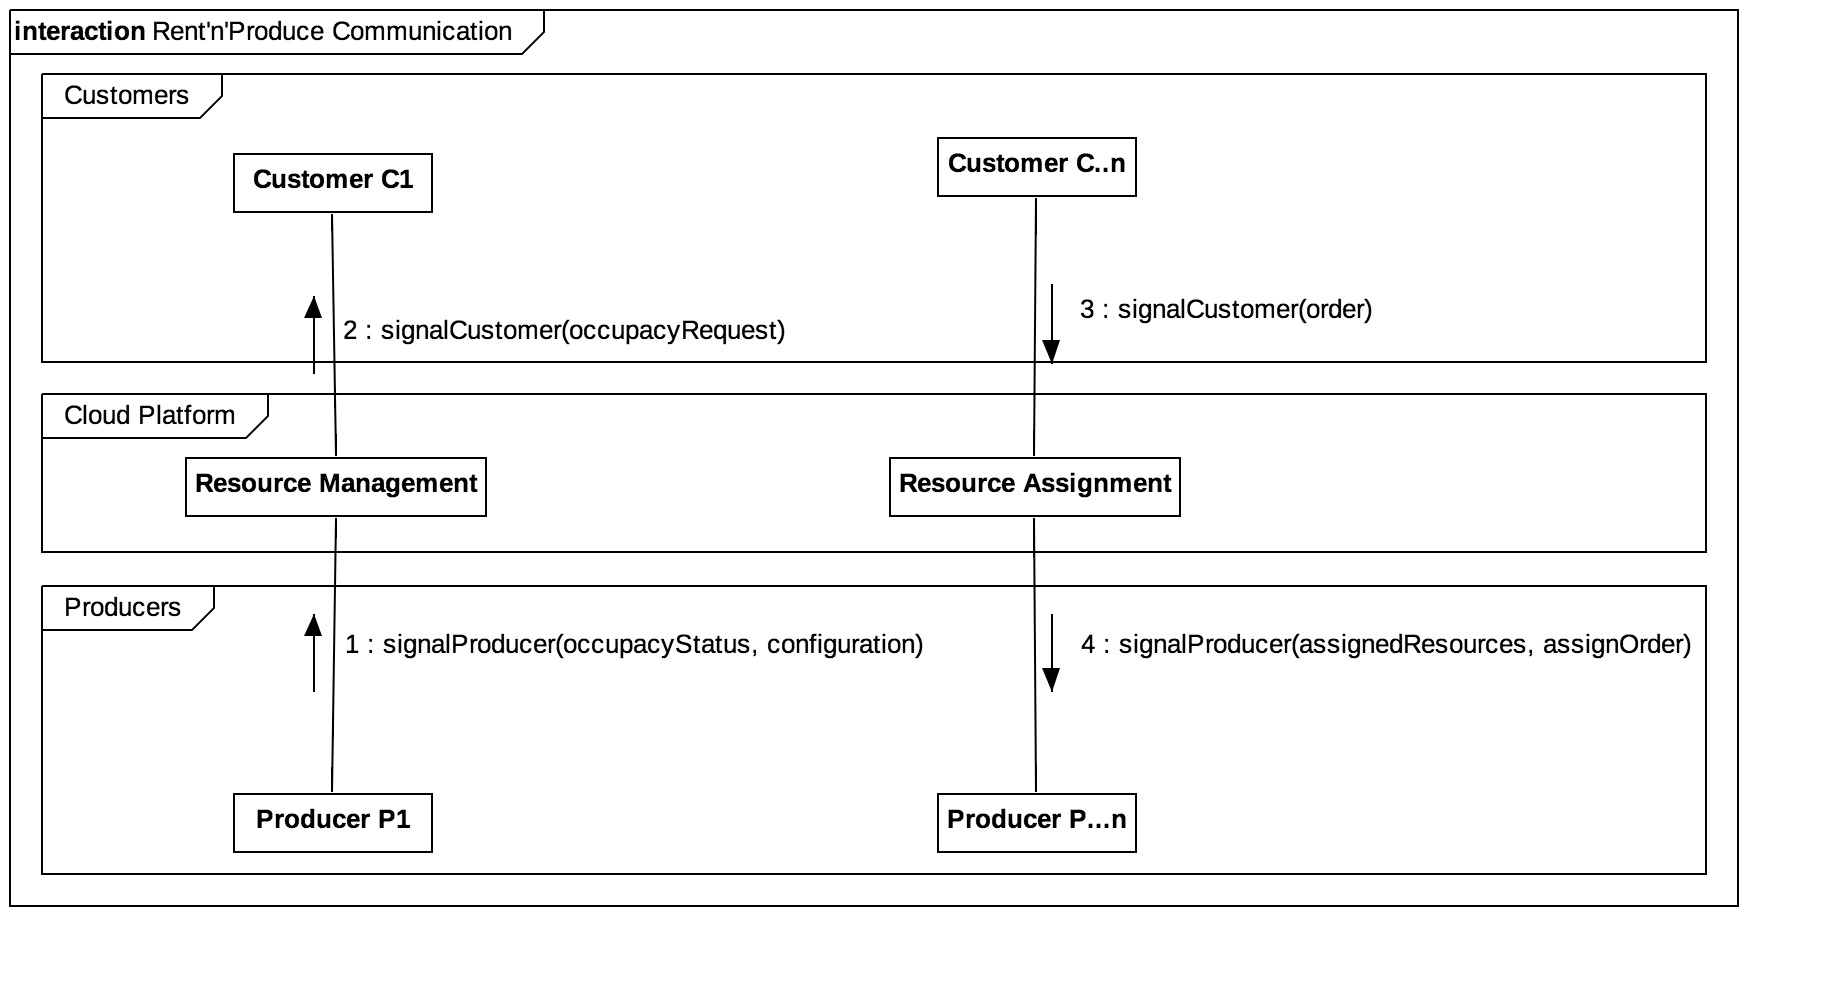
\includegraphics[width=\textwidth]{rnp_workflow.jpg}
				\caption{The workflow of the R'n'P platform adapted from~\cite{ellwein2016}.}
				\label{fig:rnp_workflow}
			\end{figure}

			Before commissioning the selected resource at the shop floor level (the production level at the Producers' manufacturing site), the production part descriptions have to go through a postprocessor and then to be adapted to the selected production resource from the resource catalog.
			This thesis deals with the transfer of existing G-Code data to a production resource.
			The postprocessing of workpiece descriptions is part of a parallel research project.

			\subsection{Initial Architecture}\label{subsec:initial_architecture}

			The architecture is based on several services which work independently of each other following a \gls{soa} approach~\cite{erl2008soa}.
			Each service is split up in a persistence layer and a business logic layer making its functionality accessible to other services using an \gls{api}.
			A simplified view on the architecture of \gls{rnp} is shown in \cref{fig:rnp_architecture} described as \gls{uml} Component Diagram following~\cite{uml2017}.
			
			The persistence layer, shown in \cref{fig:rnp_architecture}, contains the databases (\gls{sql} or \gls{nosql}) for the different services in the overall \gls{soa}. These databases offer their \gls{api}s to the Service Layer, implementing the business logic of the whole \gls{rnp} platform. As presented in \cref{fig:rnp_architecture}, the service layer is encapsulated by the \gls{api} Gateway Component, briding the \gls{api}s of the \gls{rnp} platform to the Web Interface, shown to the end-users of \gls{rnp}.

			\begin{figure}[htbp]
				\centering
				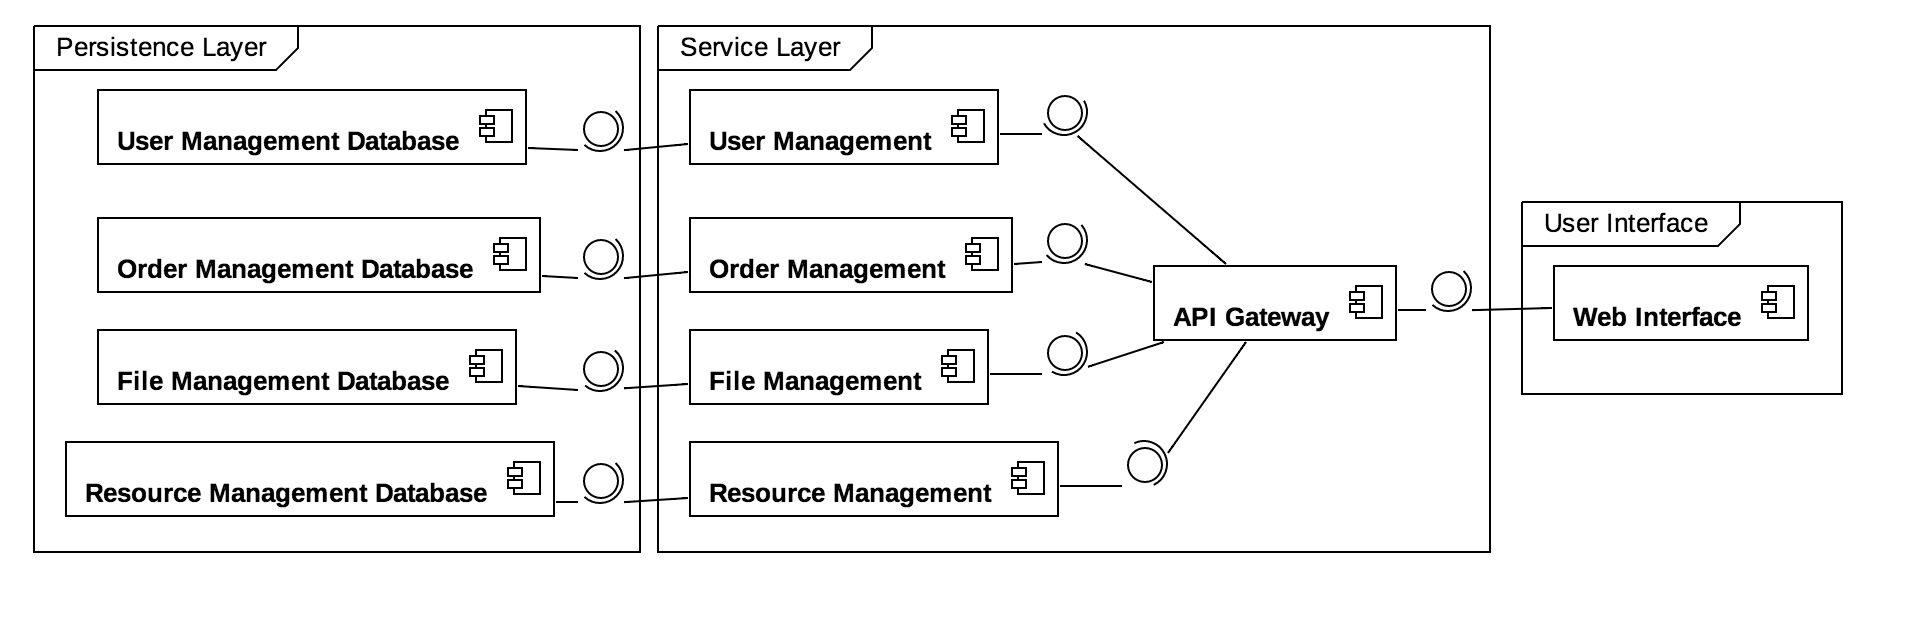
\includegraphics[width=\textwidth]{rnp_components_simplified.jpg}
				\caption{Simplified architecture of the Rent'n'Produce platform.}
				\label{fig:rnp_architecture}
			\end{figure}

			Further, every service is responsible only for one specific part of the whole platform domain(e.g., order management, user access and permission management etc.).
			Through the serverd database interface, the business logic can access the persistence layer to store and retrieve data required for domain specific operations.
			The business logic layer itself, contains all functionality provided by the platform encapsulated to different services.

			Services and databases are encapsulated in virtualization containers to ensure platform independence and the increase of maintainability~\cite{xen.17b}.
			The web interface component is the application layer which contains the \gls{ui} and the \gls{api} gateway routing all client requests to the appropriate services by its internal \gls{url} representation.

		\section{Cloud Computing}\label{sec:cloud_computing}

			By the \gls{nist} definition of cloud computing, cloud computing is a model for enabling ubiquitous, convenient, on-demand network access to a shared pool of configurable computing resources (e.g., networks, servers, storage, applications, and services) that can be rapidly provisioned and released with minimal management effort or service provider interaction~\cite{mell2011nist}.
			This cloud model is composed of five essential characteristics, three service models, and four deployment
			models~\cite{fehling2014cloud}. With regard to this work, we will focus and describe the three service models, often adapted in the manufacturing environment.

			\paragraph{\gls{saas}} The capability provided to the consumer is to use the provider's applications running on a cloud infrastructure~\cite{mell2011nist}.\footnote{A cloud infrastructure is the collection of hardware and software that enables the five essential characteristics of cloud computing. The cloud infrastructure can be viewed as containing both a physical layer and an abstraction layer~\cite{fehling2014cloud}. The physical layer consists of the hardware resources that are necessary to support the cloud services being provided, and typically includes server, storage and network components. The abstraction layer consists of the software deployed across the physical layer, which manifests the essential cloud characteristics. Conceptually the abstraction layer sits above the physical layer.}
			The applications are accessible from various client devices through either a thin client interface, such as a web browser (e.g., web-based email), or a program interface~\cite{mell2011nist}.
			The consumer does not manage or control the underlying cloud infrastructure including network, servers, operating systems, storage, or even individual application capabilities, with the possible exception of limited userspecific application configuration settings~\cite{mell2011nist}.

			\paragraph{\gls{paas}} The capability provided to the consumer is to deploy onto the cloud infrastructure consumer-created or acquired applications created using programming languages, libraries, services, and tools supported by the provider~\cite{fehling2014cloud}.\footnote{This capability does not necessarily preclude the use of compatible programming languages, libraries, services, and tools from other sources.}
			The consumer does not manage or control the underlying cloud infrastructure including network, servers, operating systems, or storage, but has control over the deployed applications and possibly configuration settings for the application-hosting environment.

			\paragraph{\gls{iaas}} The capability provided to the consumer is to provision processing, storage, networks, and other fundamental computing resources where the consumer is able to deploy and run arbitrary software, which can include operating systems and applications~\cite{leymann2011cloud}. The consumer does not manage or control the underlying cloud infrastructure but has control over operating systems, storage, and deployed applications; and possibly limited control of select networking components (e.g., host firewalls)~\cite{mell2011nist}.

			As shown in \cref{sec:rent_n_produce}, the \gls{rnp} cloud platform is built upon a \gls{iaas} layer providing its functionality over the \gls{paas} and \gls{saas} models. The goals and motivations of this work, can be related to the \gls{paas} model, as machin-tools and manufacturing sites should be provisioned over the services provided by the platform.

		\section{Cloud Manufacturing}\label{sec:cloud_manufacturing}

			With the broad adoption of cloud computing concepts and technology in the software industry, especially the use of virtualization, shared resources, outsourcing of high performance workloads, \gls{soa} and the concepts described in \cref{sec:cloud_computing}, \gls{cm} emerged and is getting adapted more and more in the production environment~\cite{he2015state}. \gls{cm} models the relocation of production resources via the internet either at times of equipment peaks or from cost reasons~\cite{wu2013cloud}. Further, \gls{cm} allows its users to access a pool of manufacturing services and resources in a flexible and location independent (only limited by the real-time connectivity required) manner, using an \gls{xaas} payment model only taking the usage time into account~\cite{macia2012cloud}.

			Services offered to the manufactures range from product design and development to manufacturing production of the requested parts~\cite{xu2012cloud}. The provided resources  are managed and encapsulated in a centralized way through the whole automation pyramid~\cite{kleinemeier2014automatisierungspyramide}.
			In a \gls{cm} system, three types of users and roles are defined -- providers, consumers and operators~\cite{wu2013cloud}.

			Providers offer manufacturing resources on the platform.
			Their roles and respective representations can vary from private customers, small business to specialized manufacturing service providers~\cite{tao2014cciot}.
			Clients occupy and use the manufacturing resources provided by the platform by paying for the usage time of the specific machine-tools~\cite{he2015state}.
			Last but not least operators are responsible for operating and maintaining the services provided on the platform as well as to deliver services which can be used by both parties mentioned above~\cite{xu2012cloud}.
			Moreover, operators are hold accountable to maintain and modernize the service stack within the platform including, architecture, technologies and security related methodologies~\cite{tedeschi2015security}.
			
			The architecture of a \gls{cm} platform shown in \cref{fig:cloud_manufacturing} in a \gls{uml}-like Interaction Diagram following~\cite{uml2017} is constructed by the following four tiers and three domains: the manufacturing resource layer, virtual service layer, global service layer and the application layer~\cite{wu2013cloud}.
			The product life cycle of manufacturing, including machine-tools, gateways and administration tools, is represented by the provider domain and offered by the manufacturing resource layer.
			Resources can either be any kind of \gls{cps} as well as generalized and abstracted manufacturing capabilities~\cite{kleinemeier2014automatisierungspyramide}.
			Manufacturing resources include for instance equipment, servers or \gls{plc} units~\cite{xu2012cloud}.
			
			Abstract manufacturing capabilities describe the ability of producers and manufacturer to offer the possibility for executing specialized, non typical tasks including the associated design, planning and management processes culminating in production site specific hardware and administration tools~\cite{he2015state}.
			The virtual service layer concludes the provider domain by abstracting the underlying manufacturing resource layer and acting as an interface for the global service layer~\cite{xu2012cloud}.
			
			Cloud deployment technologies necessary to run the whole \gls{cm} system and to bridge the provider and user domains are implemented by the global service layer.
			By mentioning cloud deployment technologies we refer to \gls{iaas} or a \gls{paas} offering, as described in~\cref{sec:cloud_computing}.
			Two operational modes are enabled for the global service layer -- complete service mode and partial service mode.
			The complete service mode orchestrates all manufacturing processes itself~\cite{xu2012cloud}.
			In the partial service mode, it is possible for providers to take control over the processes at system scope where the global service layer supports the management and organization of these processes.
			
			Finally, the application layer rounds off the \gls{cm} model by being responsible for end-user demand and manufacturing process management mapping~\cite{xu2012cloud}.
			
			\begin{figure}[htbp]
				\centering
				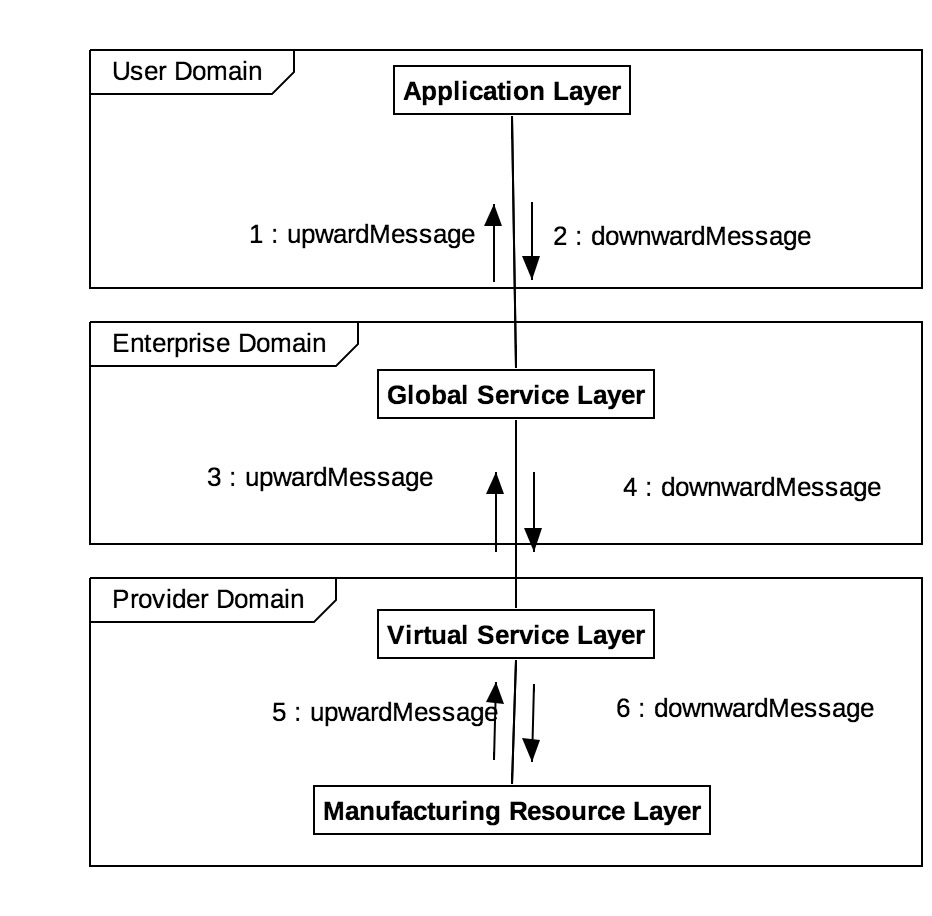
\includegraphics[width=\textwidth]{cloud_manufacturing.jpg}
				\caption{Architecture of a cloud manufacturing system adapted from~\cite{xu2012cloud}.}
				\label{fig:cloud_manufacturing}
			\end{figure}

		\section{OPC UA} \label{sec:opc_ua}

			The \gls{opcua} is the new version of the well-known \gls{opc} architecture~\cite{hadlich2006providing} originally designed by the \gls{opc} Foundation to connect industrial devices to control and supervision applications~\cite{henssen2014online}. 
			The focus of \gls{opc} is on getting access to large amounts of real-time data while ensuring performance constraints without disrupting the normal operation of the devices~\cite{candido2010soa}.
			The original \gls{opc} specifications, based on Microsofts \gls{com}, are becoming obsolete and are gradually being replaced by new interoperability standards, including web-services what led the \gls{opc} Foundation to publish a new architecture, called \gls{opcua}~\cite{hadlich2006providing}.
			
			\paragraph{Notice} The following two figures, shown in~\cref{fig:opc_ua_server_model} and~\cref{fig:opc_ua_client_model} were cited with the kind permission of the \gls{opc} Foundation to cite this images by referencing the origin \gls{opcua} Specification Part referenced in~\cite{opcfoundation2017part1}.

			\subsection{Server Model}\label{subsec:opc_ua_server_model}

				\gls{opcua} specifies the exchange of real-time information of production plant data between control devices or \gls{it} systems from different manufacturers~\cite{venkatesh2005validating}.
				The communication is established by an \textit{inverted} client-server system, where the client triggers actions on the server for automation control, and the server executes the commands on, or retrieves data from the underlying machine~\cite{imtiaz2013scalability}.
				
				\Cref{fig:opc_ua_server_model} shows the \gls{opcua} Server Model according to its specification in~\cite{opcfoundation2017part1}.
				\gls{opcua} servers include an information model that allows users to organize data and their semantics in a structured manner.
				This semantic \textit{AddressSpace} is constructed of standalone or interconnected \textit{Node}s mapped to real \gls{cps} object representatives as shown in~\cref{fig:opc_ua_server_model}.
				Furthermore, nodes can be divided into functionality and view nodes, each sort implementing different functionalities and manners of user interaction. Further, each node can be monitored and subscribed by parties of interest using the \gls{opcua} Server \gls{api} as presented at the bottom of~\cref{fig:opc_ua_server_model}.
				The information model constitutes the address spaces of \gls{opcua} servers.
				It is a fullmesh network of nodes with their properties and relations.
				
				In general, users create the information model for their \gls{opcua} servers manually at implementation time or implement vendor-specific automatism~\cite{henssen2014online}.
				A server address space consists of the following element types which are shown in \Cref{fig:opc_ua_server_model}.

				\begin{itemize}

					\item \textit{Object}: ``A \textit{Node} that represents a physical or abstract element of a system. Objects are modeled using the \gls{opcua} \textit{Object Model}. Systems, subsystems and devices are examples of Objects. An Object may be defined as an instance of an ObjectType.`'~\cite{opcfoundation2017part1}

					\item \textit{ObjectType}: ``A Node that represents the type definition
					for an Object.`'~\cite{opcfoundation2017part1}

					\item \textit{Variable}: ``A Variable is a Node that contains a value.`'~\cite{opcfoundation2017part1}

					\item \textit{VariableType}: ``Node that represents the type definition for a Variable`'~\cite{opcfoundation2018part3}

					\item \textit{DataType}: ``An instance of a DataType Node that is used together with the \textit{ValueRank} attribute to define the data type of a Variable.`'~\cite{opcfoundation2018part3}

					\item \textit{ReferenceType}: ``A Node that represents the type definition of a \textit{Reference}. The ReferenceType specifies the semantics of a Reference. The name of a ReferenceType identifies how source Nodes are related to target Nodes and generally reflects an operation between the two, such as “A Contains B”.`'~\cite{opcfoundation2017part1}

					\item \textit{Method}: ``A callable software function that is a component of an Object.`'~\cite{opcfoundation2017part1}

					\item \textit{View}: ``A specific subset of the \textit{AddressSpace} that is of interest to the \textit{Client}.`'~\cite{opcfoundation2017part1}

				\end{itemize}

				\begin{figure}[htbp]
					\centering
					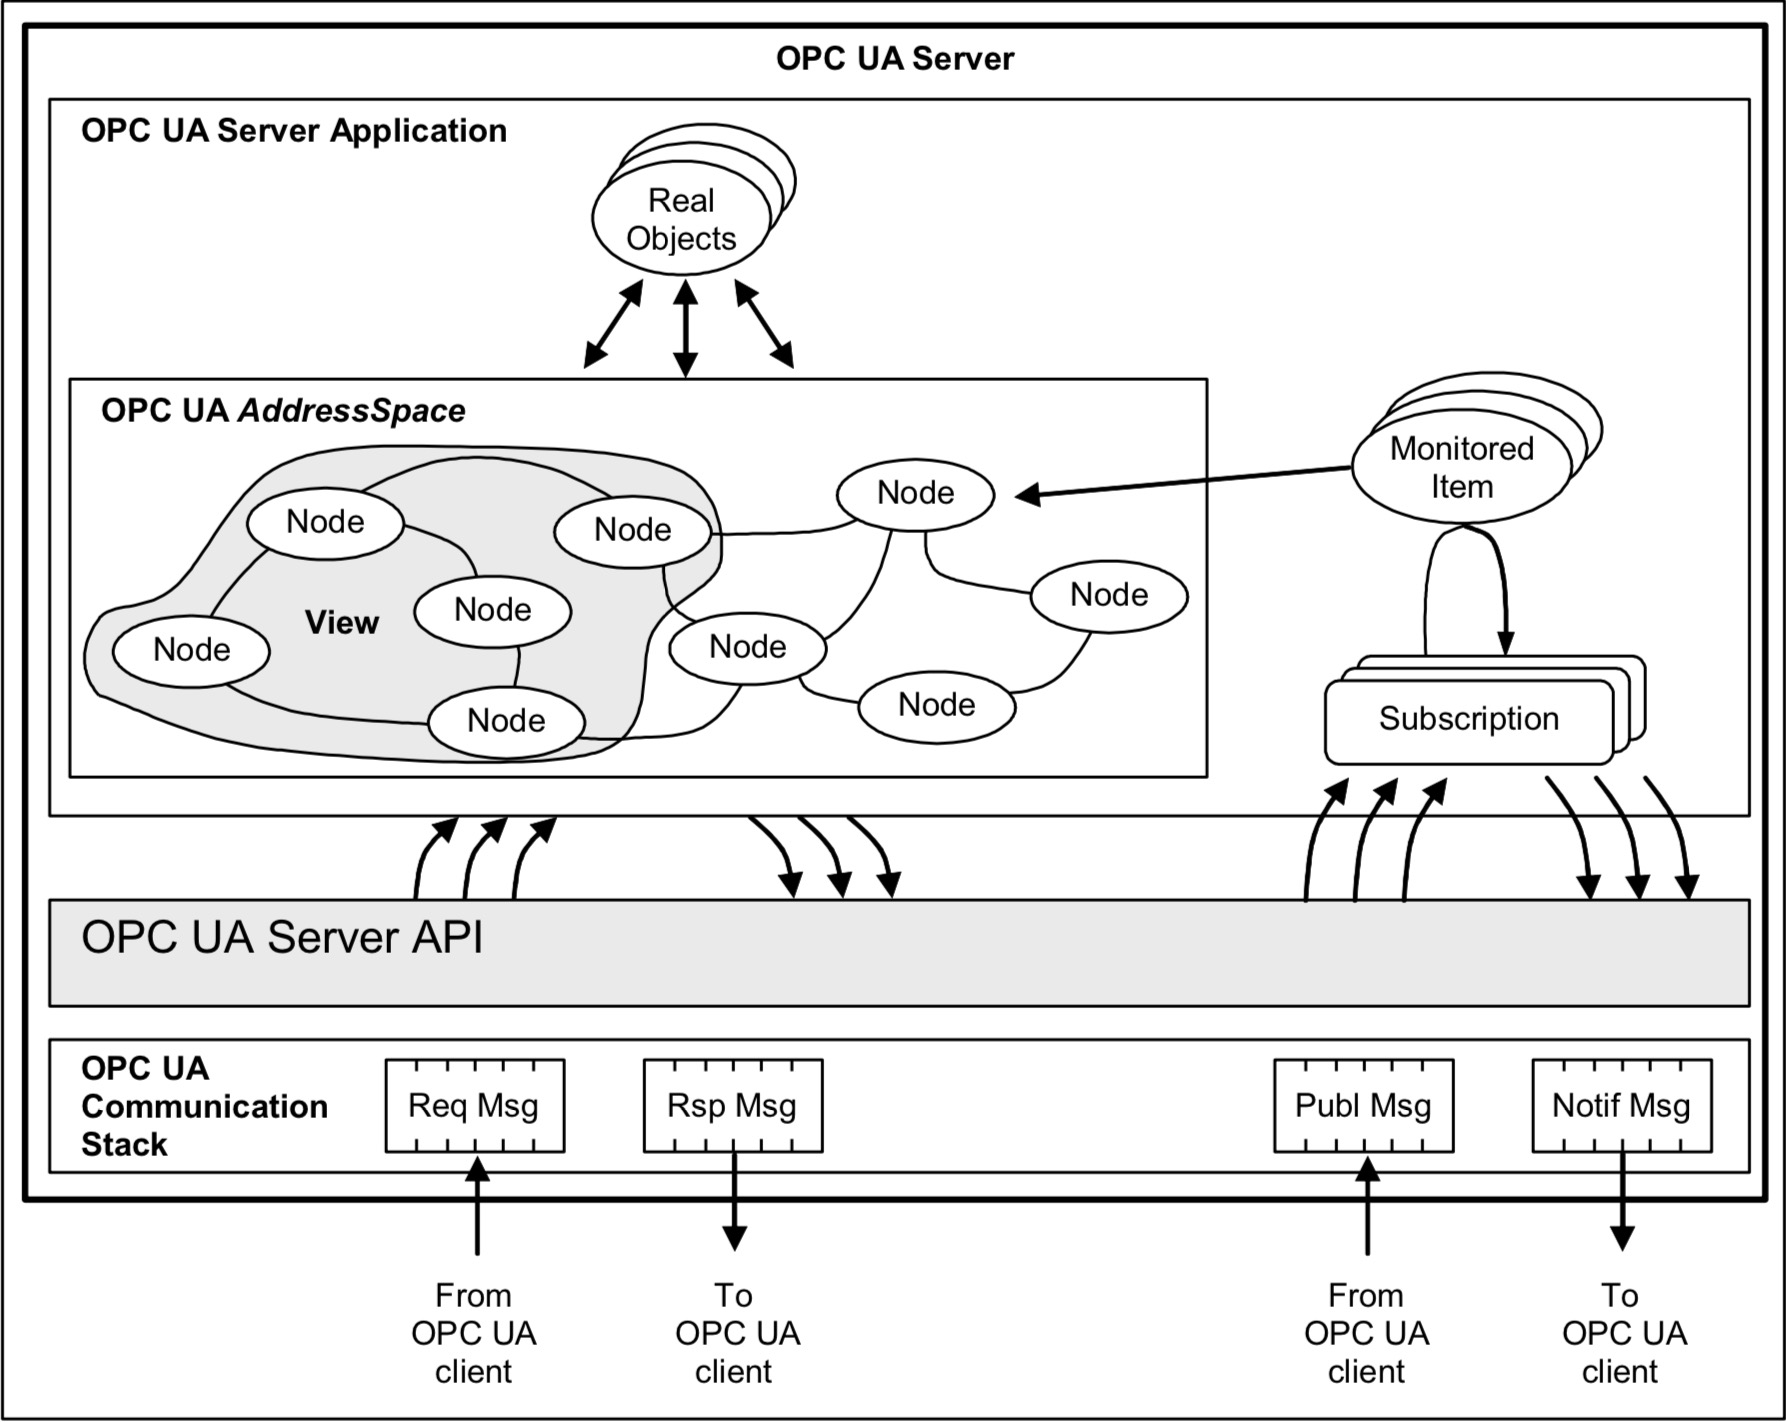
\includegraphics[width=\textwidth]{opc_ua_server_model.jpg}
					\caption{The OPC UA server architecture adapted from~\cite{opcfoundation2017part1}.}
					\label{fig:opc_ua_server_model}
				\end{figure}

			\subsection{OPC UA Client Model}\label{subsec:opc_ua_client_model}

				The \gls{opcua} Client architecture models the Client endpoint of client/server interactions.
				\Cref{fig:opc_ua_client_model} illustrates the major elements of a typical Client and how they relate to each other.
				As presented in~\cref{fig:opc_ua_client_model}, the \gls{opcua} Client is constructed by two layers -- the Client Application and the \gls{opcua} Client \gls{api}. The Client Application encapsulates the producer–consumer service functionality by accessing the underlying \gls{opcua} Client-\gls{api} following the asynchronous system designs described in~\cite{tanenbaum2007distributed}.
				
				Further, the Client Application is the code that implements the function of the Client.
				It uses the Client \gls{api} to send and receive \gls{opcua} Service requests and responses to the Server.
				The Services defined for \gls{opcua} are described in Clause 6.4 of~\cite{opcfoundation2017part4}.
				Note that the ``Client API`' is an internal interface that isolates the Client application code from an \gls{opcua} Communication Stack.
				
				The \gls{opcua} Communication Stack converts Client \gls{api} calls into Messages and sends them through the underlying communications entity to the Server at the request of the Client application.
				The \gls{opcua} Communication Stack also receives response and \textit{NotificationMessages} from the underlying communications entity and delivers them to the Client application through the Client \gls{api}.

				\begin{figure}[htbp]
					\centering
					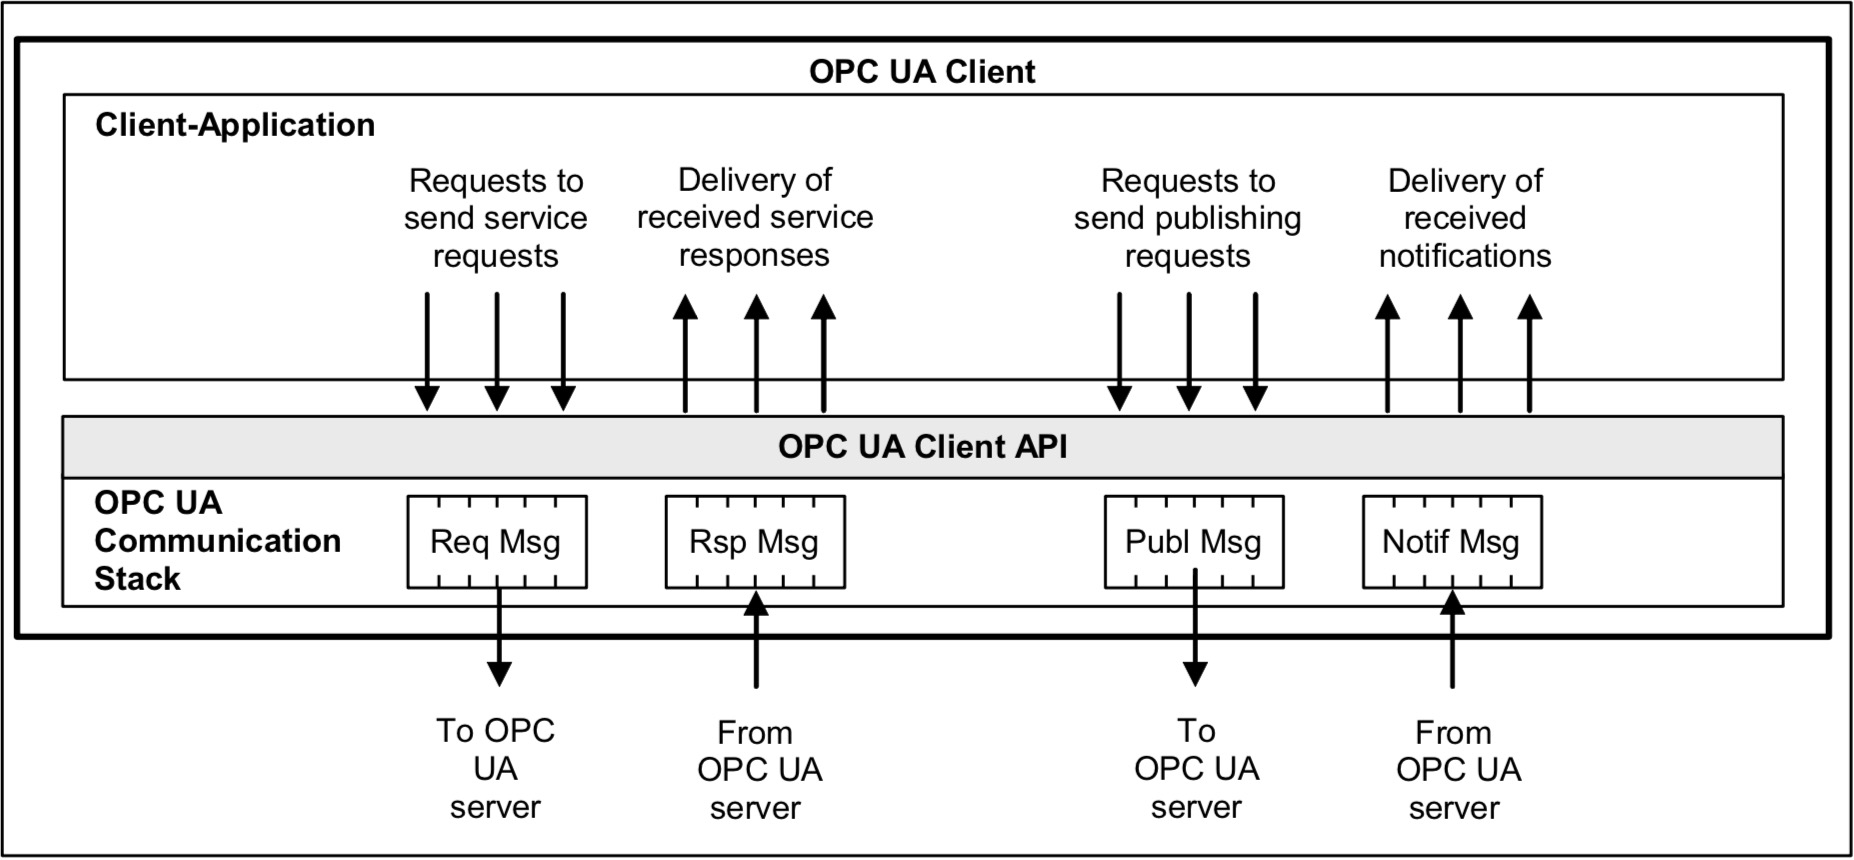
\includegraphics[width=\textwidth]{opc_ua_client_model.jpg}
					\caption{The OPC UA client architecture adapted from~\cite{opcfoundation2017part1}.}
					\label{fig:opc_ua_client_model}
				\end{figure}

	\chapter{State of the Art}\label{ch:state_of_the_art}
	
		In this chapter we cover the state-of-the-art concepts and technologies being used for the evaluation, implementation and integration of our \gls{poc}. \Cref{sec:spring_boot} introduces the Spring Boot framework for the Java~\cite{java2015} programming language. In \cref{sec:docker} we highlight the trending virtualization container technology Docker. Eclipse Milo, a Java~\cite{java2015} framework for \gls{opcua} is described in \cref{sec:eclipse_milo}. The \gls{rest} concept for \gls{api} design is covered by \cref{sec:rest}

		\section{Spring Boot}\label{sec:spring_boot}

			The \gls{soa} of the \gls{rnp} platform was realized using the Java~\cite{java2015} programming language in combination with the Spring Boot Framework\footnote{\url{https://projects.spring.io/spring-boot/}}. The framework provides enterprise ready and production based patterns and functionalities for building backend services in cloud architectures. Spring Boot provides a common abstraction layer of database entities, repositories abstracting the underlying persistence layer, services implementing the business logic and \gls{rest} controller presenting the business logic as \gls{rest}-ful \gls{api} including the mapping of different data models like \gls{json} or \gls{xml} to Java~\cite{java2015} objects.
			
			Besides its clean architectural approach, Spring Boot provides standard enterprise pattern configurations for message broker, service discovery, performance and metrics tracing as well as custom web-server configurations with little to no configuration effort.

		\section{Docker and Docker Compose}\label{sec:docker}
		
			Docker\footnote{\url{https://www.docker.com/}} is an open source project providing a systematic way to automate the faster deployment of Linux applications inside portable containers~\cite{bernstein2014containers}. 
			Basically, Docker extends \gls{lxc} with a kernel-and application-level API that together run processes in isolation: \gls{cpu}, memory, disk read and write operations, network, and so on. 
			Docker also uses namespaces to completely isolate an application’s view of the underlying operating environment, including process trees, network, user identifiers, and file systems.
			Docker containers are created using base images.
			A Docker image can include just the OS fundamentals, or it can consist of a sophisticated prebuilt application stack ready for launch. 
			When building images with Docker, each action taken (that is, command executed, such as an installation of dependencies) forms a new layer on top of the previous one. 
			Commands can be executed manually or automatically using Dockerfiles.
			
			The difference between standard hypervisor virtualization and Docker containers is shown in \cref{fig:virtualization}.
			Each block, shown in~\cref{subfig:hypervisor} and~\cref{subfig:docker} describes a physical or software layer, of the virtualization process. 
			By referencing the hardware layer, we refer to the underlying physical device either represented by a server or general computer. 
			The Host Operating system refers to the Operating System installed upon the underlying hardware architecture.
			The blocks in the first virtual machine described in~\cref{subfig:hypervisor} represents a virtualized computer, containing its own Operating System, binaries containing encapsulated system functionalities to run specific software of the Operating System and the Application as the piece of software to be run in the virtual machine.
			Analogously, these terms and symbols find their use in~\cref{subfig:docker}.
			
			\begin{figure}[htbp]
				\centering
				\begin{subfigure}{0.45\textwidth}
					\centering
					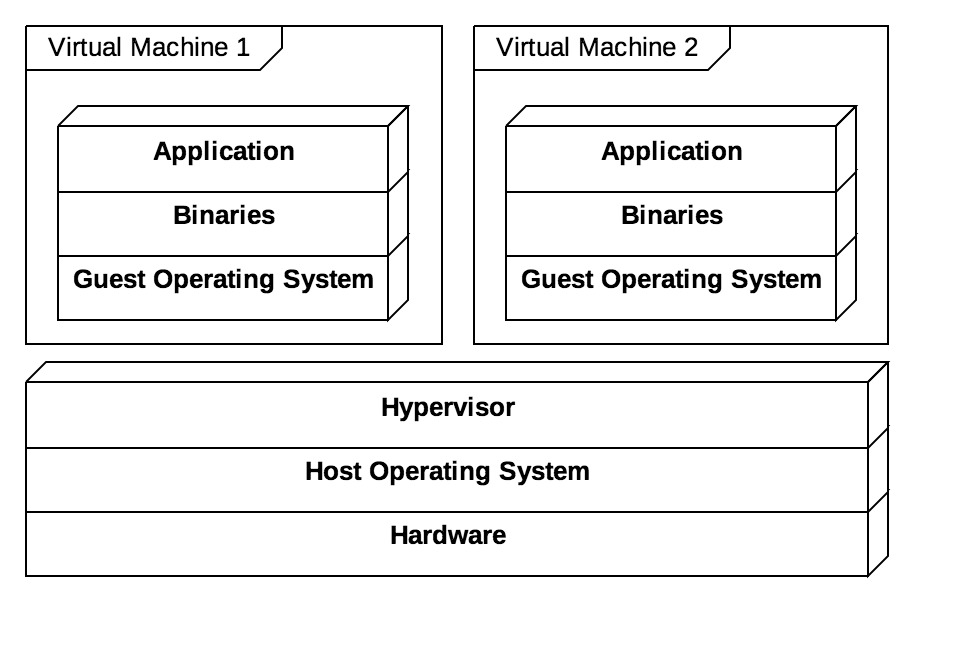
\includegraphics[width=0.9\linewidth]{virtual_hypervisor.jpg}
					\caption{A diagram showing the layers of a hzypervisor-based virtualization.}
					\label{subfig:hypervisor}
				\end{subfigure}
				\hfill
				\begin{subfigure}{0.45\textwidth}
					\centering
					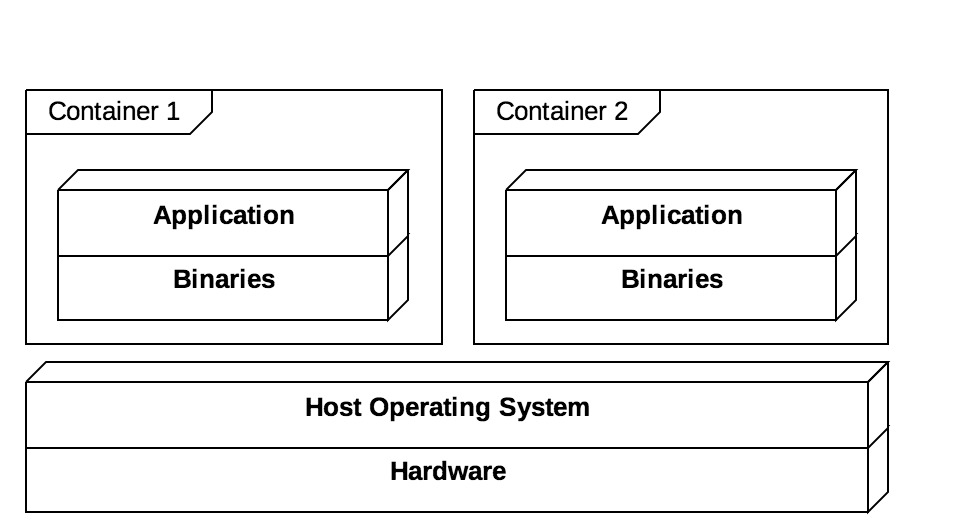
\includegraphics[width=0.9\linewidth]{virtual_docker.jpg}
					\caption{A diagram showing the layers of a Docker container virtualization.}
					\label{subfig:docker}
				\end{subfigure}
				\caption{Diagrams showing hypervisor-based and Docker virtualization.}
				\label{fig:virtualization}
			\end{figure}
			
			While standard virtualization builds each operating system itself, container rely only on the presence of the Docker Engine, encapsulating services in minimal environments.
			Docker Compose\footnote{https://docs.docker.com/compose/} is a tool for defining and running multi-container Docker applications. It offers configuration, management and orchestration utilities for container based or hybrid architectures. Further, Docker Compose can be used to deploy Docker containers and its services to different hosting environments by guaranteeing the same deployment and service architecture on each of the different environments.

		\section{Eclipse Milo}\label{sec:eclipse_milo}

			Eclipse Milo\footnote{\url{https://github.com/eclipse/milo}} is an open-source implementation of the \gls{opcua} specification written in the Java~\cite{java2015} programming language. 
			It includes a high-performance stack (channels, serialization, data structures, security) as well as client and server libraries built on top of the stack.
			While this project has existed for some time, it is new to the Eclipse foundation and is therefore considered to be in incubation\footnote{\url{https://projects.eclipse.org/proposals/milo}}.
			
			For the implementation part of this work, we will use this library as our research has shown, that Eclipse Milo implements the full \gls{opcua} specification providing simple abstraction layers to ease a simple interaction with the machine-tools and its' \gls{plc}s.

		\section{Representional State Transfer}\label{sec:rest}

			\gls{rest} is a pattern of resource operations that has emerged as a \textit{de facto} standard for service design in Web 2.0 applications~\cite{battle2008bridging}. Whereas the traditional approaches to Web Services uses full-blown remote objects with remote method invocation and encapsulated functionality, \gls{rest} deals only with data structures and the transfer of their state~\cite{fielding2000architectural}.
			
			At the core of \gls{rest} based design is a set of state transfer operations universal to any data storage and retrieval system.
			These operations, as commonly interpreted on the web, are referred to by the acronym \gls{crud}~\cite{battle2008bridging}.
			The Web 2.0 community has adopted an informal mapping of \gls{crud} operations onto the commands provided by the \gls{http} protocol: POST, GET, PUT, and DELETE, respectively. 
			These commands identify the particular \gls{crud} operation being requested of the resource identified by the \gls{url} endpoint.
			\Cref{tab:http_rest_mapping} shows the mapping between \gls{rest} and the \gls{http} protocol.
			
			\begin{table}[hbtp]
				\centering
				\caption{HTTP to REST Mapping}
				\label{tab:http_rest_mapping}
				\begin{tabular}{@{}llll@{}}
					\toprule
					\gls{crud} operations & \gls{http} command & Input format & Output format
					\\ \midrule
					Create & POST & \gls{http} Form Encoded & Status 201 CREATED
					\\ \midrule
					Read & GET & None & Determined by request headers 
					\\ \midrule
					Update & PUT & \gls{http} Form Encoded & Status 200 OK
					\\ \midrule
					Delete & DELETE & None & Status 200 OK
					\\ \bottomrule
				\end{tabular}
			\end{table}

	\chapter{State of Research} \label{ch:state_of_the_Science}

		This chapter highlights related research and work respective to this thesis. \Cref{sec:state_of_science_cloud_manufacturing} summarizes the current state of \gls{cm}. In \cref{sec:control_engineering_in_the_cloud} we give a brief overview over the state of control engineering from the cloud. We close this chapter by providing information about the current research state on \gls{m2m} communication protocols in~\cref{sec:machine_to_machine_communication}.

		\section{State of Research in Cloud Manufacturing}\label{sec:state_of_science_cloud_manufacturing}

			As a new IT paradigm, cloud computing is being increasingly adopted to transform the way that \gls{it} resources are utilised and consumed~\cite{li2010cloud}. 
			Consequently, the manufacturing industry is exploring cloud computing in order to improve existing manufacturing structures and enterprise systems, to
			share and provide on-demand networked manufacturing services, and to better satisfy specific manufacturing enterprise needs~\cite{he2015state}.
			So far researchers have proposed a number of new techniques and approaches to encapsulate various virtualized manufacturing resources and capabilities as cloud-based services and to implement enterprise \gls{cm} service frameworks and platforms~\cite{tao2011cloud}.
			
			But as the use of these new paradigms gets more and more common, challenges for \gls{cm} service models and production sites arise~\cite{brettel2014virtualization}.
			Networked manufacturing for example, lacks strong management mechanisms and efficient tools to coordinate large-scale distributed resources, services and operations~\cite{xu2012cloud}.
			
			Besides the lack of management and control mechanisms in \gls{cm} multivendor systems and heterogeneous infrastructure on production sites pose additional challenges on the \gls{cm} research field~\cite{weyer2015towards}.
			The specification of standard communication protocols and data models gains a fast growing role in the automation~\cite{jazdi2014cyber} and \gls{cm} field~\cite{wollschlaeger2017future}.
			
			Further, security gets more and more relevance in \gls{cm} field.
			In a traditional on-premise application deployment model, the sensitive data of each enterprise continues to reside within the enterprise boundary and is subject to its physical, logical and personnel security and access control policies~\cite{jeschke2017industrial}. 
			However, in the \gls{saas} model, the enterprise data is stored outside the enterprise boundary, at the \gls{saas} vendor end~\cite{subashini2011survey}.
			Consequently, the \gls{saas} vendor must adopt additional security checks to ensure data security and prevent breaches due to security vulnerabilities in the application or through malicious employees.

		\section{Control Engineering in the Cloud}\label{sec:control_engineering_in_the_cloud}

			We mentioned in~\cref{sec:state_of_science_cloud_manufacturing}, that with the emerging of cloud computing patterns in the manufacturing field, control engineers as well try to move their field of automation to the cloud.
			As discussed in~\cite{jazdi2014cyber}, an approach that implements the concept of \gls{plc} in a \gls{xaas} manner was provided by their work. 
			The result presented in ~\cite{jazdi2014cyber} is a \gls{cps} including control over \gls{plc}s, implementing concepts of cloud computing and provided using the cloud computing service models. 
			Not taking performance and real-time computing requirements into account, this paper shows that a shift to the cloud in the automation field can be realized.
			
			Another research project which has automation and control using \gls{plc}s as a focus is the project piCASSO currently researched at the \gls{isw}~\cite{kretschmer2016communication}.
			Its goal is the auto-provisioning \gls{cps} to manufacturing sites.
			A platform based on a \gls{soa}, which coordinates a robot remotely through the cloud, has been presented in~\cite{kretschmer2016communication}. 
			Showing different approaches of networking in the automation field, the results several new points of interest to researchers in this field.

		\section{Machine-to-Machine Communication}\label{sec:machine_to_machine_communication}
			
			Many \gls{cps} are sensor-rich distributed real-time embedded systems that closely interact with the physical world~\cite{kang2012rdds}. 
			In such systems, numerous entities cooperate with each other to achieve their common goals. 
			They collect data from the physical world using sensors and feed the sensor data into computing resources, which in turn make real-time decisions in cooperation by sharing data and information among participating entities.
			
			In the context of \gls{cm} and control engineering from the cloud, researchers focus on the definition of standard \gls{m2m} communication protocols tackling on exactly these problems.
			Respectively, two protocols emerged for the manufacturing field trying to fulfill the needs of manufacturers -- \gls{opcua} and \gls{dds}~\cite{jazdi2014cyber}.
			While \gls{opcua} is largely adapted by European manufacturers, \gls{dds} is more popular at manufacturers in the United States.
			\gls{opcua} builds a whole abstraction model containing, communication and data structures~\cite{candido2010soa}.
			\gls{dds} on the other hand offers a more simple and unopinionated model provided by an object definition and abstraction model.

	\chapter{Concept} \label{ch:concept}

		In this chapter, we will describe our concept for the \gls{poc} to be integrated to \gls{rnp}.
		\Cref{sec:requirements} discusses and list requirements for the infrastructure and architecture of the platform, the technology decisions taken for the \gls{poc} implementation as well as mandatory and optional features. In \Cref{sec:approach} we will highlight the implementation approach of the \gls{poc} highlighting the way we integrated the service into the platform.

		\section{Requirements} \label{sec:requirements}

			In this section, we will summarize and give an overview over the requirements, gathered from the analysis of the \gls{rnp} platform and the discussion with the research partners.
			\Cref{subsec:infrastructure} will draw out the infrastructural requirements set on this work and the kind of deployment processes targeted.
			In \cref{subsec:architecture} we will discuss the architecture, in which our \gls{poc} should be integrated following by \cref{subsec:technology} which describes the technologies to use for the implementation and integration.
			With \cref{subsec:mandatory} and \cref{subsec:optional} we conclude this chapter providing mandatory and optional Use-Cases for this work.

			\subsection{Infrastructure} \label{subsec:infrastructure}

				In \Cref{sec:rent_n_produce} we described, that the \gls{rnp} platform is built upon services following the \gls{soa} approach, where each of the services takes responsibility for one specific domain task.
				Further, every service is separated into a business logic component serving the \gls{api} for its functionality, and a persistence layer component implemented either as a \gls{sql} or \gls{nosql} database.
				Following this pattern, we deduce that the requirement will be to implement the \gls{poc} as a service, which stores the machine-tool configuration data as well as the G-Code for the production part in a database and serves its \gls{api} over a service layer component.
				Further, both components will be realized using Docker containers.
				The business logic container will register itself to the service discovery component and be routed over the \gls{api} gateway.

			\subsection{Architecture} \label{subsec:architecture}

				As shown in \Cref{subsec:infrastructure} the \gls{poc} to be realized will be packaged into a Docker container and its functionality will be split up into a persistence layer and a business logic layer.
				As the machine-tool integration represents a part of the resource service process, it doesn't need a \gls{ui} integration, as this part is already implemented in the \gls{rnp} architecture.

				More precise -- the \gls{poc} should implement an \gls{api}, which can be requested from the resource service, to trigger the production of the required parts contained in a customer order.

			\subsection{Technology} \label{subsec:technology}

				A core requirement to the \gls{poc} is the support of the \gls{opcua} protocol.
				Over \gls{opcua} the \gls{poc} should communicate with the machine-tools already registered in the resource service of the platform.
				Second requirement is the filtering and recognition of G-Code data as it will be transferred to the \gls{plc} of the machine-tool.
				For the integration to \gls{rnp}, the service should support the communication of \gls{json} over \gls{http} as well as the interaction with the service discovery server and the \gls{api} gateway.

			\subsection{Mandatory Features} \label{subsec:mandatory}

				As result of this work, we want to implement and integrate a \gls{poc} into the \gls{rnp} platform, so machine-tools can be controlled over the cloud platform.
				Therefore, we need the possibility to transfer G-Code data to the platform and from the platform down to the machine-tools already provisioned.
				Finally, we want to have the possibility to trigger the start or the stop of a part production manually or automatically by the main production process. \Cref{fig:use_cases} lists the emerged Use-Cases and shows their relation to each other.

				\begin{figure}[htbp]
					\centering
					\includegraphics[width=\textwidth]{use-cases.jpg}
					\caption{The Use-Case diagram for the Proof-of-Concept.}
					\label{fig:use_cases}
				\end{figure}

				In the following tables -- \Cref{tab:use_case_upload,tab:use_case_check_machine,tab:use_case_transfer_code,tab:use_case_production_control}) -- we will describe the Use-Case definitions for the ones shown in \cref{fig:use_cases}. The descriptions include only the regular process flow, as the side effects are described in more detail in the specification, created during this research work.

				\begin{table}[hbtp]
					\centering
					\caption{Use-Case description for the upload of G-Code.}
					\label{tab:use_case_upload}
					\newcolumntype{L}{>{\centering\arraybackslash} m{.2\linewidth} }
					\newcolumntype{R}{>{\arraybackslash} m{.7\linewidth} }
					\begin{tabular}{L R}%{c c}
					% \begin{tabular}{l p{11cm}}
						\toprule
						Name & Upload G-Code
						\\ \midrule
						Identifier & /UC-10/
						\\ \midrule
						Description & The vendor converted his \gls{cad} files into G-Code, so they can be transferred to the machine-tool.
						\\ \midrule
						Actors & \begin{enumerate}\item A \gls{rnp} platform user with the vendor role. \item The \gls{opcua} Client Service.\end{enumerate}
						\\ \midrule
						Trigger & The vendor has prepared the G-Code and wants to transfer it to the machine-tool.
						\\ \midrule
						Level & User-View
						\\ \midrule
						Invariants & \begin{enumerate}\item The user stays logged in and keeps his OAuth2-Token with the appropriate scope. \item The uploaded files have not been changed in format, type or content.\end{enumerate}
						\\ \midrule
						Preconditions &
						\begin{enumerate}
							\item The user is already logged in to the system using his web-browser and his session is assigned with an OAuth2 Token including the scopes \textit{user}, \textit{customer} and \textit{vendor}.
							\item The user has the G-Code to be uploaded.
							\item The G-Code has the MIME-Type \textit{application/x-netcdf}.
							\item The user knows the identifier for the order, the G-Code is for.
						\end{enumerate}
						\\ \midrule
						\begin{tabular}{c c} 1 & User \end{tabular} & The user uploads the G-Code using an HTTP-POST request to the \gls{opcua} Client Service.
						\\ \midrule
						\begin{tabular}{c c} 2 & System \end{tabular} & The systems persists the G-Code categorized under its order identifier and responds to the user with an HTTP-201 CREATED response containing order identifier and the production part identifier.
						\\ \midrule
						Postconditions & The G-Code has been persisted to the system. From the technical point of view, the service responds with an HTTP-201 CREATED Status. The user can download the file over the same \gls{api} by providing the production part id. The G-Code file has not been manipulated after the upload.
						\\ \bottomrule
					\end{tabular}
				\end{table}

				\begin{table}[hbtp]
					\centering
					\caption{Use-Case description for the retrieval of the current machine-tool status.}
					\label{tab:use_case_check_machine}
					\newcolumntype{L}{>{\centering\arraybackslash} m{.3\linewidth} }
					\newcolumntype{R}{>{\arraybackslash} m{.6\linewidth} }
					\begin{tabular}{L R}%{c c}
					% \begin{tabular}{l p{9cm}}
						\toprule
						Name & Request machine-tool status
						\\ \midrule
						Identifier & /UC-20/
						\\ \midrule
						Description & The service is able to request the current status of the machine-tool using the \gls{opcua} protocol. The service should only request, if a machine-tool is prepared for production and does not deliver any error states.
						\\ \midrule
						Actors & \begin{enumerate}\item The \gls{opcua} Client Service. \item The machine-tool to be requested.\end{enumerate}
						\\ \midrule
						Trigger & Use-Cases including this Use-Case have been triggered as shown in~\cref{fig:use_cases}.
						\\ \midrule
						Level & Technical View
						\\ \midrule
						Invariants & This Use-Case describes only the retrieval of \gls{opcua} specific information. As long as the protocol and correction are correct, this Use-Case doesn't have any invariants.
						\\ \midrule
						Preconditions &
						\begin{enumerate}
							\item The \gls{opcua} Client Service established and holds a connection to the \gls{opcua} server of the machine-tool.
							\item The machine-tool is available over Ethernet and \gls{opcua}.
						\end{enumerate}
						\\ \midrule
						\begin{tabular}{c c} 1 & \gls{opcua} Client Service \end{tabular} & The \gls{opcua} Client Service requests one of the states from the machine-tool: \begin{enumerate}
							\item Is the machine-tool currently in an error state?
							\item Is the machine-tool ready to produce a part (e.g., material preparared and machine-tool loaded)?
							\item Is the machine-tool currently producing a part?
						\end{enumerate}
						\\ \midrule
						\begin{tabular}{c c} 2 & Machine-Tool \end{tabular} & The \gls{opcua} Server of the machine-tool responds to the requests of the client service.
						\\ \midrule
						Postconditions & The \gls{opcua} Client Service gathered the requested data from the machine-tool. This data can now be used for further production process steps.
						\\ \bottomrule
					\end{tabular}
				\end{table}

				\begin{table}[hbtp]
					\centering
					\caption{Use-Case description for transfer of G-Code to the machine-tool.}
					\label{tab:use_case_transfer_code}
					\newcolumntype{L}{>{\centering\arraybackslash} m{.3\linewidth} }
					\newcolumntype{R}{>{\arraybackslash} m{.6\linewidth} }
					\begin{tabular}{L R}%{c c}
					% \begin{tabular}{l p{10cm}}
						\toprule
						Name & Transfer G-Code to a Machine-Tool
						\\ \midrule
						Identifier & /UC-21/
						\\ \midrule
						Description & The vendor can transfer previously uploaded G-Code (as described in \cref{tab:use_case_upload}) to the machine-tool.
						\\ \midrule
						Actors & A \gls{rnp} platform user with the vendor role, the \gls{opcua} Client Service and the machine-tool the data should be transferred to.
						\\ \midrule
						Trigger & The vendor has uploaded G-Code to the system and wants to transfer it to a machine-tool.
						\\ \midrule
						Level & User-View
						\\ \midrule
						Invariants & The transferred G-Code stays persisted in the database and will not be modified. The transferred data doesn't override data already existing on the machine-tool control units.
						\\ \midrule
						Preconditions & The user is already logged in to the system using his web-browser and his session is assigned with an OAuth2 Token including the scopes \textit{user}, \textit{customer} and \textit{vendor}. G-Code has been transferred as described in~\cref{tab:use_case_upload}.
						\\ \midrule
						\begin{tabular}{c c} 1 & User \end{tabular} & The user requests the Client-Service with an HTTP-POST method containing the identifiers of the part to be produced and the producing machine-tool.
						\\ \midrule
						\begin{tabular}{c c} 2 & System \end{tabular} & The Client-Service checks the requested machine-tool for its current state as described in~\cref{tab:use_case_check_machine}.
						\\ \midrule
						\begin{tabular}{c c} 3 & System \end{tabular} & The Client-Service loads the G-Code for the part from the database.
						\\ \midrule
						\begin{tabular}{c c} 4 & System \end{tabular} & The Client-Service creates an \gls{opcua} connection with the Server on the machine-tool and sends the G-Code data.
						\\ \midrule
						\begin{tabular}{c c} 5 & The Machine-Tool \end{tabular} & The \gls{opcua} Server on the machine-tool receives the request, and stores the G-Code in the AddressSpace to a new file and loads it to the \gls{nc} of the machine-tool. Finally, a response, that the persistence was successful is sent back to the Client-Service.
						\\ \midrule
						\begin{tabular}{c c} 6 & System \end{tabular} & The Client-Service informs the user, that the transfer was successful by responding with an HTTP-200 OK status.
						\\ \midrule
						Postconditions & The G-Code has been transferred to the machine-tool and into its \gls{nc}. The user is informed that the transfer was successful and the user can continue the usage of the platform. G-Code is now a new File in the \gls{opcua} name space and can be used to produce the part.
						\\ \bottomrule
					\end{tabular}
				\end{table}

				\begin{table}[hbtp]
					\centering
					\caption{Use-Case description for the production control of the machine-tool.}
					\label{tab:use_case_production_control}
					\newcolumntype{L}{>{\centering\arraybackslash} m{.3\linewidth} }
					\newcolumntype{R}{>{\arraybackslash} m{.6\linewidth} }
					\begin{tabular}{L R}%{c c}
					% \begin{tabular}{l p{9cm}}
						\toprule
						Name & Start and Stop a part production
						\\ \midrule
						Identifier & /UC-22/
						\\ \midrule
						Description & G-Code data has been successfully transferred to a machine-tool. This G-Code should now be run to produce a part.
						\\ \midrule
						Actors & The \gls{opcua} Client-Service of the \gls{rnp} platform, as well as the control composite of the \gls{opcua} Server, the \gls{plc} and \gls{nc} of the machine-tool as the second actor.
						\\ \midrule
						Trigger & G-Code has been transferred to the machine-tool and now the part production should either be started or stopped.
						\\ \midrule
						Level & Technical View
						\\ \midrule
						Invariants & The G-Code transferred to the machine-tool stays in the same location of the \gls{plc} and \gls{nc} after the production is started or stopped. The machine-tool stays connected to the \gls{rnp} platform during the whole process.
						\\ \midrule
						Preconditions & The G-Code was properly transferred to the machine-tool as described in~\cref{tab:use_case_upload}. The \gls{opcua} Server and the machine itself are connected with the \gls{rnp} platform. The machine-tool is not in an error state as described in~\cref{tab:use_case_check_machine}.
						\\ \midrule
						\begin{tabular}{c c} 1 & \gls{opcua} Client-Service \end{tabular} & The Client-Service triggers the start or the stop of the production.
						\\ \midrule
						\begin{tabular}{c c} 2 & The machine-tool \end{tabular} & The machine-tool loads the G-Code and produces the part or stops its current production, not going into an error state.
						\\ \midrule
						\begin{tabular}{c c} 3 & \gls{opcua} Server \end{tabular} & The server registers the processes of the machine-tool and sends it to the message broker of the \gls{rnp} platform over a response to the \gls{opcua} Client-Service of the platform.
						\\ \midrule
						Postconditions & The part has been produced or the production process of the machine-tool has been stopped. The current state of the machine-tool can be monitored over the \gls{opcua} Client-Service of the \gls{rnp} platform.
						\\ \bottomrule
					\end{tabular}
				\end{table}

			\subsection{Optional Use-Cases} \label{subsec:optional}

				Besides the requirements defined to validate the \gls{poc} created in this work, we defined several optional Use-Cases to extend the capacity of the \gls{poc} which could be implemented during this work, or providing inspiration for future research on this matter.
				The optional Use-Cases pointed out during the research phase are described below in hastily manner giving space for requirement changes and other input and ideas coming from future research:

				\begin{enumerate}

					\item More than the control over the \gls{opcua} Client-Service of the \gls{rnp} platform developed during this work, we could image to transfer signals in form of visual information to the \gls{hmi} of the machine-tool. With this Use-Case we could give workers at the production site of the machine-tool the possibility to interact with the system and visually monitor the current state of the whole manufacturing process.

					\item At the state of this research, the machine-tool will be integrated only by pre configured data from the manufacturing. Allowing an auto-provisioning of the machine-tools could increase the productivity of manufacturers, as we could get to a very homogeneous production environment.

					\item We can imagine, that it could be useful to attach a monitoring or machine learning component to the service to be implemented. With a Bid Data approach we could deliver more insights on the machine to the manufacturer increasing productivity and the whole manufacturing site performance.

				\end{enumerate}

		\section{Approach} \label{sec:approach}

			With the requirements pointed out in \cref{sec:requirements} we will now present the approach used to implement and integrate the desired \gls{poc} into the \gls{rnp} platform. Using the defined requirements and Use-Cases in \cref{sec:requirements} as well as relying on the research foundations highlighted in \cref{ch:foundations} we will test the \gls{poc} against these. The developed \gls{poc} should be a service, independent of the \gls{rnp} platform to ensure a possible use on every \gls{cm} platform working with the \gls{opcua} protocol.

			\subsection{Integration} \label{subsec:integration}

				As we distilled from the platform analysis and defined in the requirements, we will package our \gls{poc} as a service, following the \gls{soa} principles into two Docker virtualization containers. One container will contain the business logic of the \gls{poc} and serve its \gls{rest}-ful \gls{api}. A second container will serve the \gls{sql} database using PostgreSQL\footnote{\url{https://www.postgresql.org/}} as the \gls{rdbms}.
				The \gls{poc} itself will communicate with the \gls{rnp} platform by registering itself to the service discovery of the platform and being routable through the \gls{api} gateway already implemented as the edge entry point of the platform.
				The binding with the machine-tool for the \gls{poc} will be done using an external \gls{url} of the \gls{opcua} Server of the machine-tool.

			\subsection{Target Architecture} \label{subsec:target_architecture}

				As shown in \cref{fig:poc_integration_diagram}, the \gls{poc} will offer an \gls{api} to the \gls{rnp} platform to gather data and control the bound machine-tool following the approach described in \cref{subsec:integration}. The component diagram shows, that following the \gls{soa} architecture of the \gls{rnp} platform, the service can be integrated
				seamlessly.

				\begin{figure}[htbp]
					\centering
					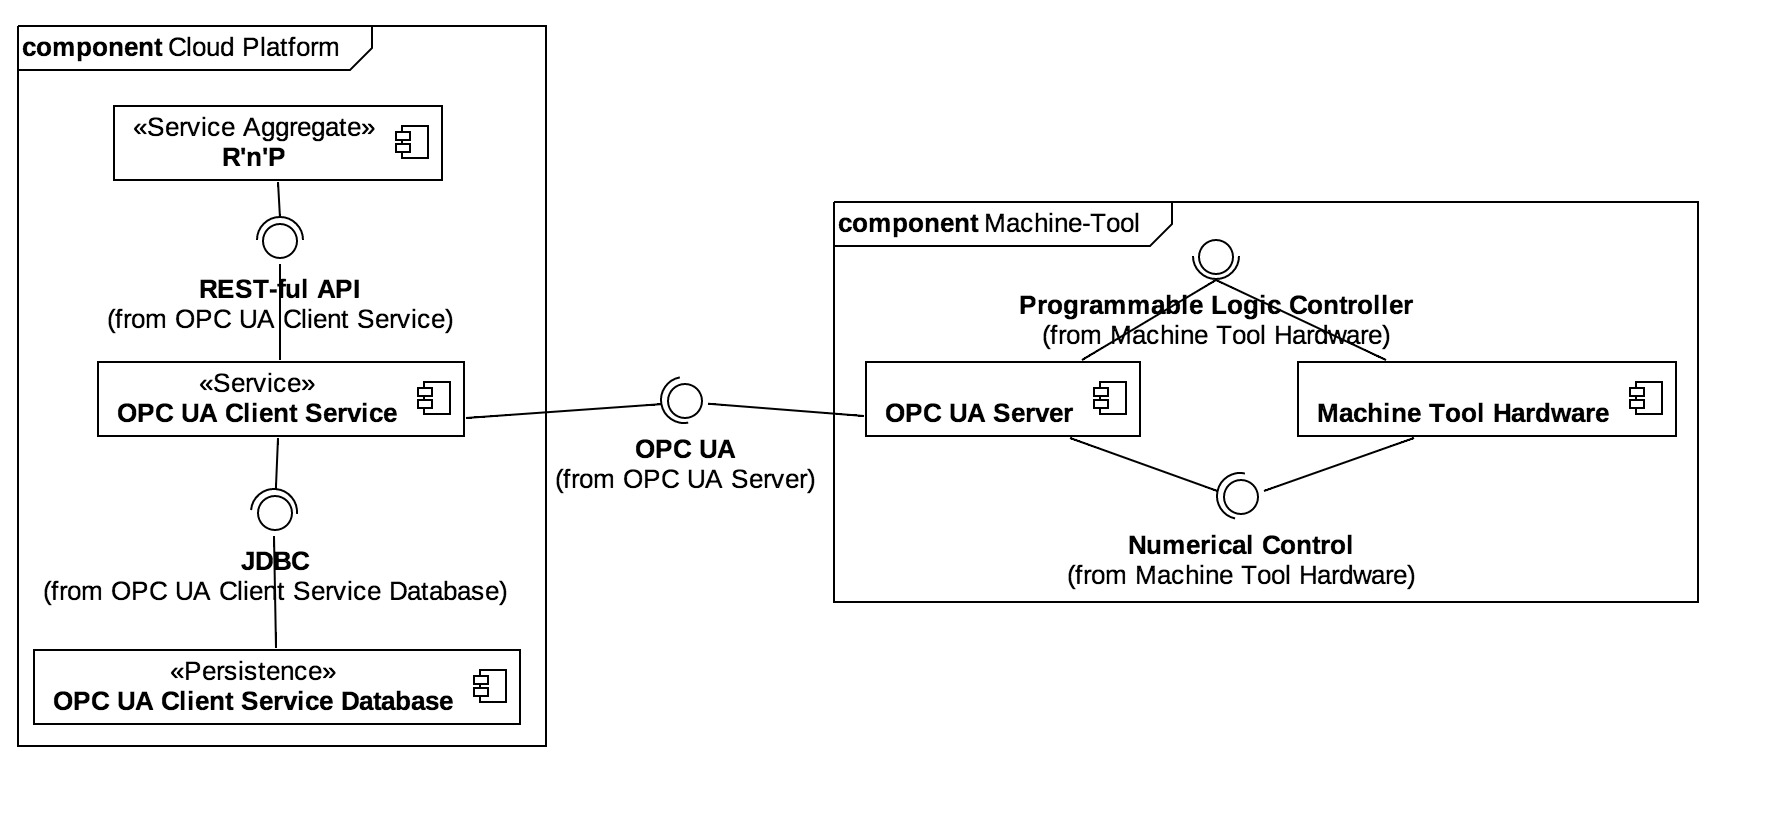
\includegraphics[width=\textwidth]{poc_integration_diagram.jpg}
					\caption{The component diagram of the integration of the \gls{poc}.}
					\label{fig:poc_integration_diagram}
				\end{figure}

				As presented in \cref{fig:poc_integration_diagram} \gls{poc} service communicates with and controls the machine-tool only addressing its \gls{opcua} server. The machine-tool itself can be abstracted into three sub components: the \gls{opcua} server running on the controlling industrial computer attached to the physical machine-tool, the \gls{plc} and the \gls{nc} as physical parts of the machine-tool.

				The \gls{opcua} Server receives client requests and commands and transfers them to the \gls{plc} unit of the machine-tool. This abstraction layer ensures, that standard requests and commands sent to the server, can be translated without the knowledge of the Client of specific machine-tool configurations.

				The \gls{plc} of the machine-tool is responsible for the physical and electrical control of the manufacturing and machine-tool processes. It can execute control commands like data gathering from the machine-tool state, start- and stop of the production and transfer data to the \gls{nc}. Processing of production parts data, planing of the milling routes for example and executing the part production is handled by the \gls{nc}. Production data is loaded from and to the \gls{nc} via the \gls{plc} and the current state is transferred to the \gls{plc} in real-time ensuring a correct monitoring of every production process.

				Making use of the \gls{opcua} specification, we can integrate the \gls{poc} and the machine-tool without adding too much of abstraction layers keeping the architecture clean, understandable and maintainable without loads of effort.

			\subsection{Services} \label{subsec:services}

				After describing the high level integration process, we now highlight the services, and \gls{api}s provided by the \gls{poc}. \cref{fig:poc_service_diagram} shows of which services and what kind of services, the \gls{poc} will be implemented. Each part of the functionality will be bound into a four tier composite -- the Entity representation of the domain specific objects to be persisted to the database, a Repository layer making database queries available using the Spring Boot JPA interface of the Entity, a Service layer implementing the business logic of the specific functionality and finally a Spring Boot \gls{rest} Controller wrapping the Service layer functionality into a \gls{rest}-ful \gls{api} also handling the mapping of \gls{json} objects to Java~\cite{java2015} Entities.

				\begin{figure}[htbp]
					\centering
					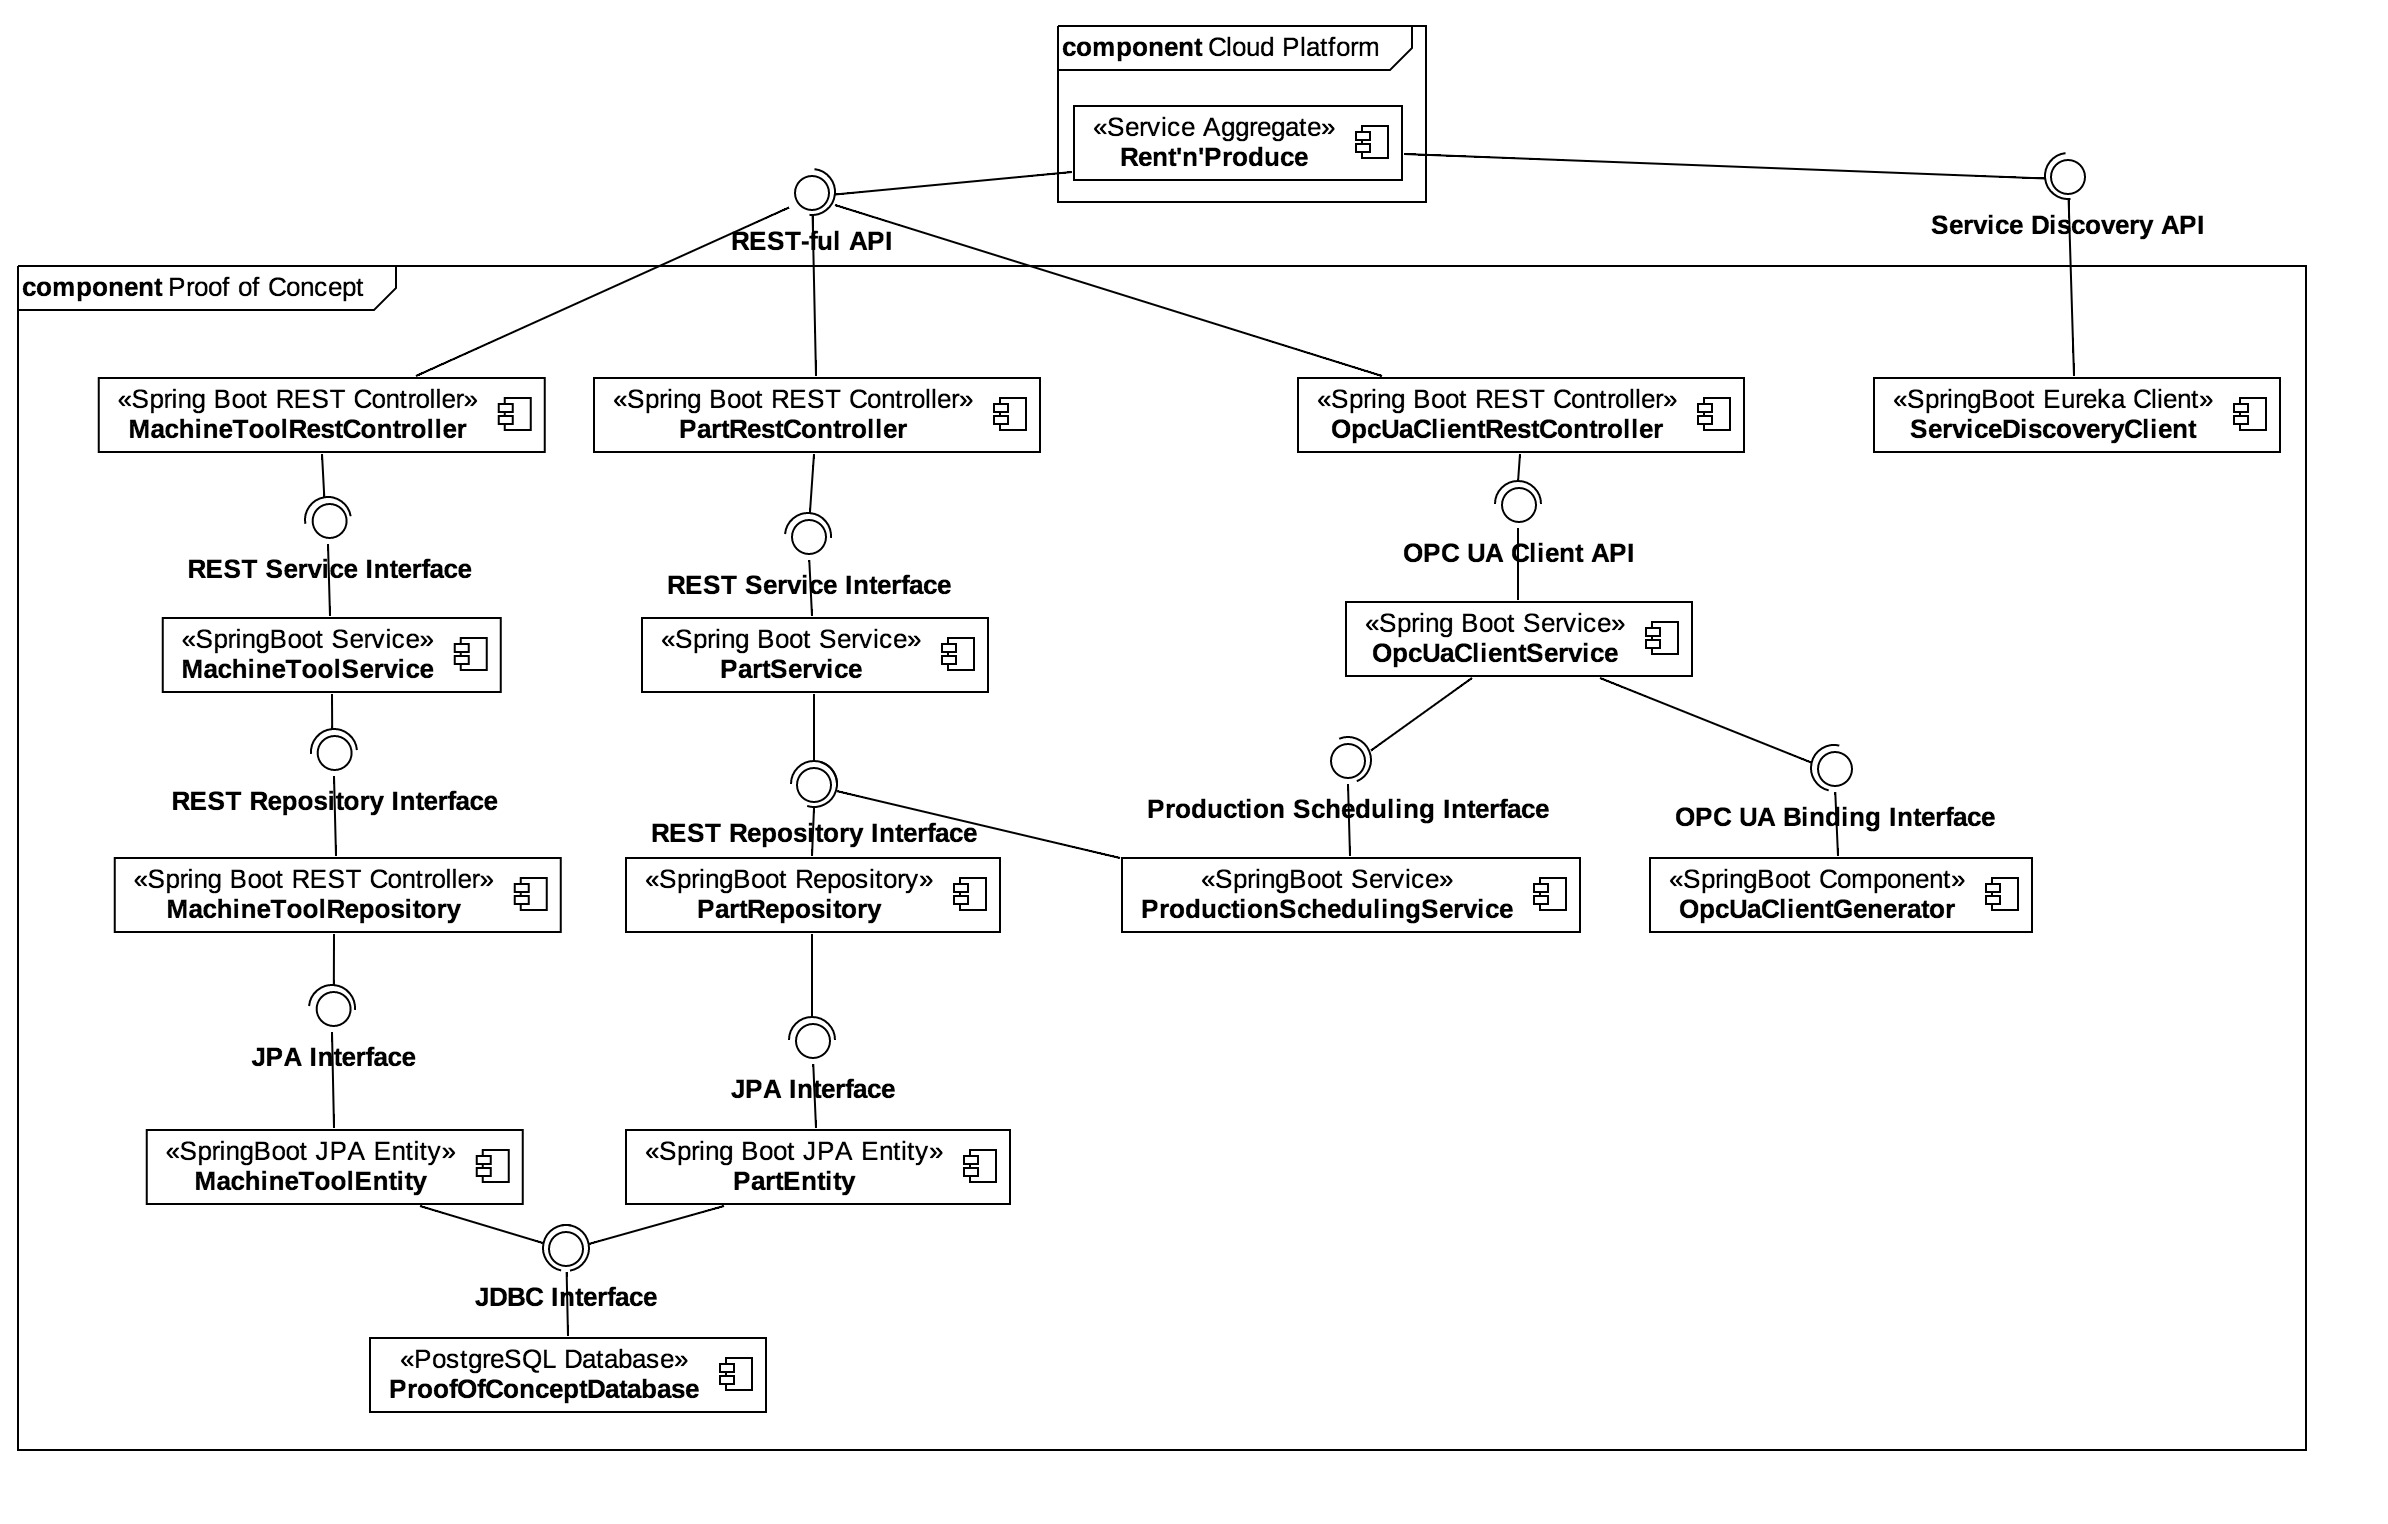
\includegraphics[width=\textwidth]{poc_services.jpg}
					\caption{The component diagram describing service details of the \gls{poc}.}
					\label{fig:poc_service_diagram}
				\end{figure}

				On the left side of \cref{fig:poc_service_diagram} we see the described blocks serving the \gls{api}s to persist, retrieve and manipulate data of the production part and machine tool domain entities. These \gls{api}s are responsible for persisting new machnine-tools and configurations to the system as well as the persistence of the parts to be produced with their G-Code data and production dates to allow automatically or manual scheduling of the production processes. As the Service Discovery and the \gls{api} gateway of the \gls{rnp} produce are tightly bound, offering the \gls{api} to the Service Discovery, the \gls{poc} is automatically able to be routed through the \gls{api} gateway, discovered and requested by other services of the platform using both, the \gls{api} gateway and the Service Discovery, and to be auto-scalled by the underlying Docker Engine and the deployment with the Docker-Compose Container orchestration mechanisms.

				Further, \cref{fig:poc_service_diagram} presents on the right site the core functionality of the \gls{poc}.
				The Service Discovery Client binds the \gls{poc} to the Service Discovery Server of the platform, allowing to be seamlessly integrated into the platform.
				The \gls{opcua} Client Service implements the connection to the machine-tools, retrieved from the part data and the machine-tool Entity representation.
				On the other hand, the Client Service creates the connection, using the provided Client Generator, implementing a generic connection utility for security credentials, machnine-tool data and further required information to establish a clean connection. Finally, the \gls{opcua} Client Service can produce parts automatically, by triggering the Scheduling Service to retrieve the production date and time of the part to be produced next, and comparing to the system time, triggering the automatic start of a part production as the machine-tool is available and its state is not an error state.
				The Service functionality is made public by a single \gls{api} wrapper.
				We note, that the Client Service functionality is implemented in an asynchronous manner, as data transfer and part production can take quite a long time and the client should not wait so long to inform the user about a success or a failure. Therefore, the client will respond to the user at the moment, as all paradigms for a successful file transfer or production start are given. After the \gls{http} response, the user is informed over the event messages, sent to the message broker, available at global scope for the entire \gls{rnp} platform. Using this approach, we can ensure a user experience with no deadlocks and paralleling production processes.

			\subsection{Workflow Concept} \label{subsec:workflow_concept}

				Targeting our goal to be able to upload G-Code to the \gls{rnp} platform, to transfer the G-Code to a connected machine-tool and to produce the production part described with the G-Code, we will now describe the general workflow of the whole part production of the \gls{poc} using the \gls{opcua} protocol.
				User interactions with the \gls{poc} are realized by triggering the \gls{rest}-ful \gls{api} provided by the \gls{poc} using \gls{json} over \gls{http} as communication base.
				System information related to other components of the system and to the user are implemented using asynchronous messaging with the \gls{amqp} provided by the global message broker of the \gls{rnp} platform.
				Communication between the system and the machine-tool, which should produce the part is managed with the \gls{opcua} protocol as described in \cref{sec:opc_ua}.
				We refer as the basic workflow of the \gls{poc} as the implementation of the Use-Cases to upload G-Code, request the current machine-tool state, the transfer of G-Code to the machine-tool and the start of the part production, as shown in \cref{tab:use_case_upload,tab:use_case_check_machine,tab:use_case_transfer_code,tab:use_case_production_control}.

				In \cref{fig:poc_workflow_diagram} we describe in the first steps the Use-Case, that the user has G-Code prepared from the \gls{cad} file of the part to be produced. The user sends an \gls{http}-POST request in \gls{json} format to the system, containing his authentication header, the G-Code to be uploaded to the system, the identifier of the machine-tool that should produce the part\footnote{We want to mention, that by sending the identifier of a selected machine-tool to produce specific part, the service checks if the catalog contains multiple machine-tools with the same configuration parameters. If this is the case, one machine-tool that is available at the production time of the part will be selected to produce the part.} and the production time of the part.

				Receiving the user request, the service checks if the request is valid and if the user has the required permissions to perform the \gls{api} call. If the requirements are not met in the request it will be rejected and the user gets an information in the \gls{api} response. If the request has been sent correctly, the service starts to check the machine-tool catalog and the configurations of the production process.

				\begin{figure}[htbp]
					\centering
					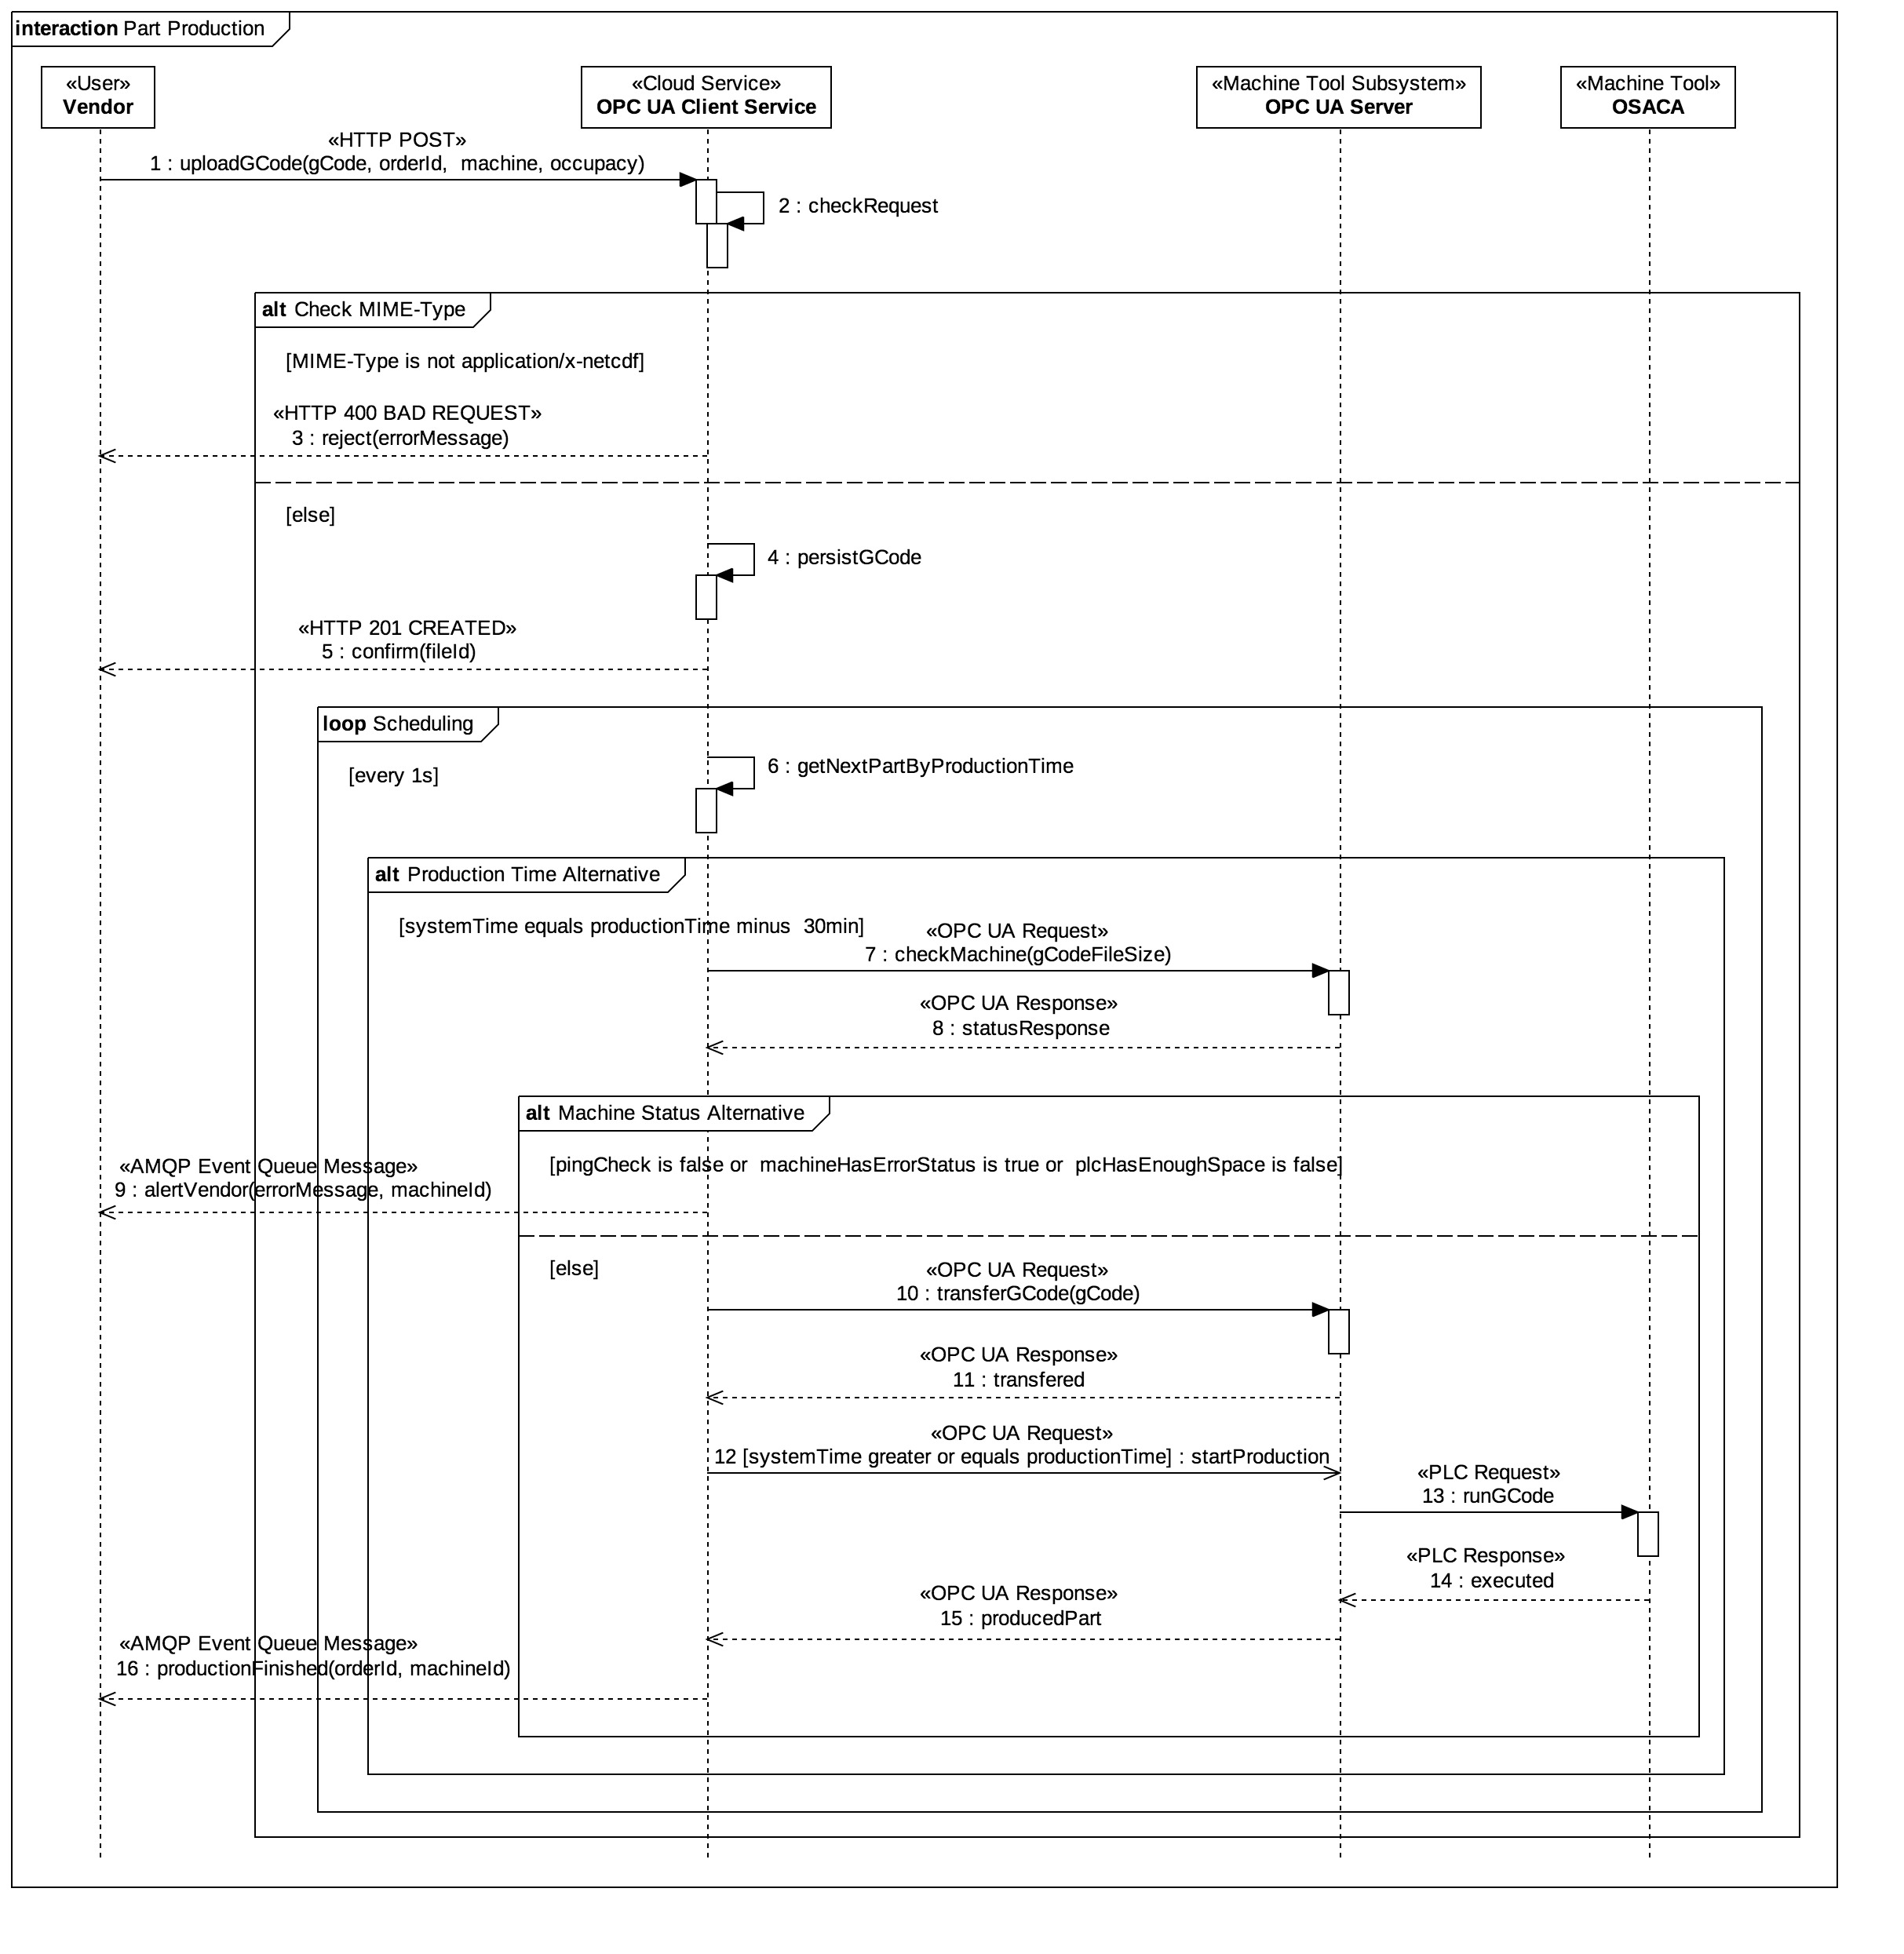
\includegraphics[width=\textwidth]{part_production_sequence.jpg}
					\caption{Sequence diagram of the general part production process.}
					\label{fig:poc_workflow_diagram}
				\end{figure}

				If the configuration check and the following persistence of the production part and the machine-tool relation is successful, the user request is finished with a positive response and the automatic production process starts.
				The \gls{poc} checks every second, if the order of the parts to be produced is still consistent with production dates of all valid parts in the database. Is the current system time 30 minutes away from the start of the production, the system begins to transfer the G-Code data of the part to the machine-tool by firstly checking the current machine status (not including that the machine tool can be in production mode) as shown in \cref{tab:use_case_check_machine} and begins to transfer the G-Code data to the machine-tool as described in \cref{tab:use_case_transfer_code}.

				In the case, that the production paradigms are not met, the part will be rescheduled in the database to a deferred state and the manufacturer user is informed over an asynchronous message. In the other case that, all requirements are met, the production is started at the moment the system times equals the part production time. After the successful production of the part, the user is again informed over an asynchronous message.

				By describing the workflow shown in \cref{fig:poc_workflow_diagram} we handled all the requirements and Use-Cases described in \cref{sec:requirements}. Further we have highlighted that with the prior knowledge of the concepts described in \cref{ch:foundations} and the analysis of the system, we are able to model an automatic manufacturing process only relying on Open Source Technologies and the \gls{opcua} specification. In \cref{subsec:machine_tool_intergation} we will describe the machine-tool integration between the \gls{rnp} \gls{opcua} Client Service running in the cloud and the machine-tool itself to finalize the whole manufacturing process model.

			\subsection{Machine Tool Integration} \label{subsec:machine_tool_intergation}

				In \cref{subsec:workflow_concept} we presented the concept of the regular workflow for the automatic part production of our \gls{poc}. The description of the machine-tool integration side will finalize our model. The machine-tool will be integrated using its \gls{opcua} server.

				To check the machine-tool status, the client will read the current status data from the servers AddressSpace. These variables are set machine-tool specific and have to be determined for each server and machine-tool. For our \gls{poc} we will use the Beckhoff TwinCAT V3\footnote{\url{http://www.beckhoff.de/twincat3/}} control and \gls{opcua} server for demonstration and testing purposes and describe machine-tool specific commands using its specification defined in ~\cite{twincat2018}. The machine-tool for experiment purposes is a 3-axis milling machine provided by the \gls{isw}.

				The machine-tool status check is handled, using the standard \gls{opcua} client read function to determine, if the current machine state in the TwinCAT NameSpace is not of type \textit{AlarmType} in the \textit{UA\_StatusCode}. If no entry is currently provided for any of these types (described in Clause 8.2 of~\cite{twincat2018}) under the \textit{DeviceState} \gls{opcua} Object, the machine-tool has no error state and it leaves us to check, if the machine-tool is ready for part production or currently producing a part. The check if the machine-tool is currently producing a part, is done by checking, if any motion state changes arrived in the \textit{UA\_NodeGetHandleList} as if the production is ready, the event list is empty. Connectivity analysis of the machine-tool is handled implicitly as every read request of data requires a valid \gls{opcua} connection.

				Transferring a G-Code data file is handled by the \gls{poc} as follows using the provided functionality of the TwinCAT control unit and its \gls{opcua} Server:

				\begin{enumerate}
					\item The Client connects to the Server and checks if a program with the file name of the G-Code data already exists.
					\item If the G-Code already exists, the client appends temporary the system date to the file name and triggers the creation of a new \textit{UA\_FileType} in the programs folder for the project.
					\item After the empty file is created on the Server side, the client writes a byte stream into the file created using an \textit{UA\_Write} command to the server.
					\item Finishing the write command, the client triggers the naming of the file and the setting of project specific parameters.
				\end{enumerate}

				In the last step of the part production, as we now transferred the G-Code down to the \gls{plc} of the machine-tool using the \gls{opcua} server, we can now start the part production at the required time. Therefore, we trigger the \gls{opcua} server to create a new \textit{Task} in the TwinCAT automation project and execute it using the predefined workflow in \textit{UA\_Method} and \textit{UA\_Function} calls in the \gls{plc}.

				We denote, that we have to keep in mind, that for a machine-tool independent implementation, the \gls{opcua} server configurations and provided methods have to be homogeneously distributed over all machine-tools connected with the platform. More information on that follows in~\cref{sec:limitations}.

			\subsection{Security} \label{subsec:security}

				Besides the implementation of an automatic part production from the cloud, we should keep in mind, that business relevant data passes the processes from to the cloud, and down to the machine-tools of manufacturers, which leads us to the need of securing the data transfer and providing some kind of user access and permission control. As the field of security is far beyond the scope of this work, we want to describe some security approaches taken to secure the platform and the developed \gls{poc} only by touching the huge field of security in the manufacturing environment.

				First of all, the Client service in the cloud should check, if the data uploaded is really G-Code on no other format. Therefore, a G-Code parsing library is used to check the content of the G-Code data and to prove, that no other parameters are set. Further, a header check is required to determine the file format for parsing. If not each of these criteria is given, the file upload is aborted, ensuring no harmful data can be uploaded to the cloud.

				User access and permissions to access the \gls{api} is regulated by the Oauth2 protocol to handle user access sessions to the system. Only users with the appropriate access tokens can send requests to each service of the \gls{rnp} platform, including the \gls{poc}. Besides that, only the manufacturers identified by their tokens, can see the machine-tools they own and trigger the data transfer to them, which builds an additional security layer.

				Finally, the access on machine-tool level is secured using the \gls{opcua} security mechanisms. Each \gls{opcua} server of each machine-tool has a fine granulated access and method call description secured using identity certificates. The \gls{poc} initializes the certificate negotiation at the first time, the machine-tool is bound to the cloud platform. The service itself can only add G-Code files to the machine-tool \gls{plc} but can't remove data from or interrupt native \gls{plc} implementations.

	\chapter{Discussion} \label{ch:discusion}

		In this chapter, we will compare the concept and approach described in \cref{ch:concept} to the actual implementation and experiment work with our \gls{poc}. \Cref{sec:integration_results} will describe the result of how well the \gls{poc} could be integrated into the \gls{rnp} platform. Comparison of the self defined Use-Cases and goals with the actual implementation will be described in \cref{sec:use_cases_implementation}. Finally, limitations of the \gls{poc} and the whole approach are shown in \cref{sec:limitations} closing this chapter.

		\section{Integration Results}\label{sec:integration_results}

			After implementing the \gls{poc} with the requirements defined in \cref{sec:requirements} and the goals of this work listed in~\cref{sec:goals} in mind, the developed \gls{poc} could be totally integrated into the \gls{rnp} platform as planned. By using the Docker container runtime, the \gls{poc} could be integrated into any \gls{paas} solution and architecture, running on Docker Engine as container and orchestration platform.

			The implemented \gls{rest}-ful \gls{api} encapsulates all functionalities of the \gls{poc} and provides it to any third-party service, that is able to communicate using \gls{json} over \gls{http} and receive messages from an \gls{amqp} message broker. The database serving the \gls{poc} service can be interchanged to any \gls{sql} database as well as additional components like chaching, searching and logging utilities can be added with low effort and cost.

			As the OAtuh2 protocol is provider independent, custom implementations of a user access and permission management providers can be added or replace the current implementation at no effort and cost. Same criteria were met for the service discovery and \gls{api} gateway cloud computing patterns.
			The \gls{opcua} functionalities of the service are encapsulated to the service as well, making it manufacturer independent as long as the manufacturers' machine-tools support the \gls{opcua} protocol.

			Summing up the results, the \gls{poc} could be implemented and integrated seamlessly to the \gls{rnp} platform. With this result, we fulfill our requirement, that the \gls{poc} should be platform independent and serving a standard \gls{api}.

		\section{Use-Case Implementation}\label{sec:use_cases_implementation}

			After we defined the Use-Cases in \cref{subsec:mandatory}, we will prove each of them against the actual implementation of the \gls{poc}. This will serve as the real proof of our concept and unveil limitations of our approach.

			\subsection{Uploading of G-Code}\label{subsec:uploading_g_code}

				By offering the \gls{api} to upload simple files in the G-Code file format, this Use-Case is proofed by our \gls{poc}. Files can be uploaded and before persisting the files for a specific production step, the system checks, if the header parameters for the file type and the file content itself is G-Code data. Requests with any other type of data will be rejected. Exception handling if the information provided or requested by the is invalid is implemented too.

			\subsection{Machine-Tool Status Checking}\label{subsec:machine_tool_status_checking}

				The implemented \gls{poc} provides an \gls{api} for checking the current machine-tool status. Behind this \gls{api}, a generic \gls{opcua} connection utility generates UA connections for the provided machine-tools already persisted in the database beforehand. The \gls{api} could be extended by enumerations, to provide granulated access to the specific values requested by the user.

				An asynchronous connection is built each time the \gls{opcua} \gls{api} of the \gls{poc} is triggered, checking the following parameters:

				\begin{enumerate}
					\item Is the machine-tool available over Ethernet?
					\item Is the machine-tool available for a connection over \gls{opcua}?
					\item Is the machine-tool currently in an \gls{opcua} error state?
				\end{enumerate}

				As the last parameter is machine-tool specific and relies on the \gls{opcua} server implementation on the machine-tool, this point will be discussed in \cref{sec:limitations}. Nevertheless, the \gls{poc} provides the \gls{api} as described in the Use-Case shown in~\cref{tab:use_case_check_machine}, which leads us to the conclusion, that the \gls{poc} provides the functionality required.

			\subsection{G-Code Transfer}\label{subsec:g_code_transfer}

				With the possibilities implemented as described in \cref{subsec:machine_tool_status_checking}, the machine-tool status can be checked, before a previously uploaded G-Code file can be transferred to the machine-tool to produce the part. The approach described in \cref{subsec:machine_tool_intergation} is the standard path to complete a file transfer following the \gls{opcua} specification.

				After monitoring and logging the requests sent in each step of the transfer workflow described in \cref{fig:poc_workflow_diagram}, we ensure that the implemented functionality is correct as it reflects the suggested \gls{opcua} process and data flow. An interesting recognition taken from the experiment to transfer G-Code data to the TwinCAT \gls{plc} has been, that even if the TwinCAT offers the described \gls{api}, the \gls{opcua} server of the machine-tool responded, that the requested function is not available and returns a StatusCode showing a correct request but bad response. This led to the conclusion, that the function call has to be implemented on the server side of the connection. This knowledge contradicts our concept to create a machine-tool independent service for file transfer and production. Limitation will be disscussed deeper in \cref{sec:limitations}.

			\subsection{Part Production}\label{subsec:part_production}

				As the requirements for a file transfer have not been met completely as mentioned in \cref{subsec:g_code_transfer}, the part production out of the G-Code could not be tested in the whole scope. We implemented a test controller to read and set status data on the TwinCAT \gls{plc} using its \gls{opcua} Server. As expected, these data were available and the StatusCodes and Types could be read without any further complications.

				Assuming, that the parameters could be read and written under the fitting \textit{UserWriteMask} we expect that with a proper configuration of the \gls{opcua} server of the \gls{plc} the start and stop of the production, would simply trigger already implemented functions on the \gls{plc} to pursue with the part production.

		\section{Limitations}\label{sec:limitations}

			As a result of our test of the \gls{poc} against the Use-Cases and requirements define beforehand, we learned, that the requirements were totally met. Further, we learned, that the implementation is theoretically independent of the underlying machine-tool and control units, as they offer the \gls{opcua} interfaces to handle a file transfer and machine-tool status checking. The issues have been, that behind the interface, the implementation on the machine-tool side is either not existent, or varies in a strong manner, leaving it to the manufacturers to configure their \gls{plc}s to their needs.

			Further limitations have been found during the research phase of the project. Dependent on the real-time requirements of the system, it could be possible, that the \gls{poc} doesn't fit these requirements as a data, signal and file transfer to the control units can take a while, missing the required real-time signal slots. Further, the \gls{poc} totally depends on a prior knowledge of the \gls{opcua} addresses and security configurations from the manufacturer as that these have to be provided during the persistence of machine-tools to the \gls{rnp} platform. Finally, an automatic provisioning of the machine-tools by their \gls{opcua} addresses is still not possible, as the types, versions and software states of the manufacturers \gls{plc}s can be highly heterogeneous, making it impossible for the \gls{poc} to know which kind of services the \gls{plc} really supports, making the need of a kind of gateway inevitable.

	\chapter{Conclusion and Future Work} \label{ch:conclusion_and_future_work}

		This Chapter provides a short summary of this work in~\cref{sec:conclusion}. In addition, future work on the system is proposed and use-cases are discussed in~\cref{sec:future_work}.

		\section{Conclusion}\label{sec:conclusion}

			In this work, an approach for the automated part production in the manufacturing field using the \gls{rnp} platform and the \gls{opcua} specification has been proposed. To accomplish this task, a concept has been derived from the analysis of the \gls{rnp} cloud manufacturing platform and its missing functionalities at the beginning of this work.

			First, foundations of \gls{cm} and the \gls{opcua} specification were presented. This provided a base for examining the state of the art, the state of the research and related work.

			With the aid of observations made in foundational as well as related work, an approach implementing a working \gls{poc} which seamlessly integrates into the \gls{rnp} platform was presented. The \gls{poc} encapsulates its functionality in a Docker container and provides it through a \gls{rest}-ful \gls{api} to be platform and language independent. Further persistence and management models were developed and integrated into the \gls{poc}. The \gls{opcua} and machine-tool integration was implemented following the principles of the \gls{opcua} specification. We learned that even if the cloud-based client implements just the basic \gls{opcua} functionality, it is still a matter of machine-tool configuration, making a truly machine-tool independent solution not possible with this \gls{poc}. Finally, we summarized the limitations of the \gls{poc} and the approach and provided information about the architecture and implementation for future research work.

		\section{Future Work}\label{sec:future_work}

			The presented approach is not totally machine-tool independent, as it relies on the server-side implementations provided as \gls{opcua} interfaces. For a better handling and analyzation of manufacturing sites topologies, we suggest providing a supplement service for \textit{scanning} the manufacturing sites allowing the service to get insights to the individual topologies.

			In addition, the \gls{poc} currently expects from the users, that they exactly know the addresses and configuration details of their machine-tools. One could image to make research on manufacturing site provisioning and automatic registration of machine-tools to the platform with ideal information about the possible manufacturing processes.
			At last, future research could extend the current \gls{rnp} platform and especially the \gls{poc}, to implement a central authorization and certificate management service for all machine-tools of a production site. This would ease the configuration and access management of each machine-tool and lead to a higher security level of the whole platform.

	\clearpage

	% \printindex

	\printbibliography

	All links were last followed on \today.

	\pagestyle{empty}
	\renewcommand*{\chapterpagestyle}{empty}
	\Versicherung

\end{document}
